%%%%%%%%%%%%%%%%%%%%%%%%%%%%%%%%%%%%%%%%%%%%%%%%%%%%%%%%%%%%%%%%%%%%%%%%%%%%%%%%%%
% \documentclass[12pt,papel,twoside]{ibtesis}
\documentclass[12pt,screen,twoside,pagebackref]{ibtesis}
% \documentclass[12pt,papel,singlespace,oneside]{ibtesis}
% \documentclass[12pt,papel,preprint,singlespace,oneside]{ibtesis}


%%%%%%%%%%%%%%%%%%%%% Paquetes extra %%%%%%%%%%%%%%%%%%%%%%%%%%%%%%%%%%%%%%%%%%%
% Por conveniencia: aqu\'{\i} puede cargar todos los paquetes y definir los comandos 
% que necesite
\usepackage{ibextra}
%\usepackage[spanish,es-nodecimaldot]{babel}
\usepackage{amsfonts}
\usepackage{algpseudocode}
\usepackage{algorithm}
\usepackage{graphicx}
\usepackage{bm}
\usepackage{booktabs}

%\includeonly{datos_utilizados, hp_greedy}
%%%%%%%%%%%%%%%%%%%%%%%%%%%%%%%%%%%%%%%%%%%%%%%%%%%%%%%%%%%%%%%%%%%%%%%%%%%%%%%%

\renewcommand{\algorithmicrequire}{\textbf{Input:}}
\renewcommand{\algorithmicensure}{\textbf{Output:}}
\floatname{algorithm}{Algoritmo}

%%%%%%%%%%%%%%%%%%%%% Informacion sobre la tesis %%%%%%%%%%%%%%%%%%%%%%%%%%%%%%%
\title{Criterios b\'{a}sicos para la presentaci\'{o}n de la tesis en el Instituto Balseiro Tanto de doctorado como de maestr\'{\i}a}
\author{J. Autor}
\director{Dr.~J.~Director}
\codirector{Dr.~J.~Otro m\'{a}s}
\carrera{Tesis Licenciatura en F\'{\i}sica}
\grado{Doctorando}
\laboratorio{Colisiones At\'{o}micas -- Centro At\'{o}mico Bariloche}
\jurado{Dr.~J.~J.~Jurado (Instituto Balseiro) \\ 
Dr.~Segundo Jurado (Universidad Nacional de Cuyo)\\ 
Dr.~J.~Otro Jurado (Univ. Nac. de LaCalle)\\
Dr.~J.~L\'{o}pez Jurado (Univ. Nac. de Mar del Plata)\\
Dr.~U.~Amigo (Instituto Balseiro, Centro At\'{o}mico Bariloche)}
\palabrasclave{formato de Tesis, Lineamientos de escritura, Instituto Balseiro}
\keywords{Thesis format, Templates, Instituto Balseiro}
% Si queremos poner la fecha manualmente:
% \date{Diciembre de 2099}

%%%%%%%%%%%%%%%%%%%%%%%%%%%%%%%%%%%%%%%%%%%%%%%%%%%%%%%%%%%%%%%%%%%%%%%%%%%%%%%%
%\titlepagefalse % Si no quiere compilar la portada descomente esta linea
%\includeonly{apendices} % Compilar s\'{o}lo estos archivos 
\graphicspath{{figs/}} % Lugar donde encontrar las figuras generales (se puede poner uno en cada cap{\'{\i}}tulo)
%%%%%%%%%%%%%%%%%%%%%%%%%%%%%%%%%%%%%%%%%%%%%%%%%%%%%%%%%%%%%%%%%%%%%%%%%%%%%%%%


\begin{document}

% Dentro del environment 'preliminary' va:
% la dedicatoria, resumen, abstract, indices

\begin{preliminary}

% Escriba su dedicatoria
\dedicatoria{
A mi familia\\
A mis amigos\\
A todos los que me conocen\\
A toda esa otra gente que no
}

%%% \'{I}ndices %%%%

\begin{abreviaturas}
                                %Abreviaturas
\end{abreviaturas}

\tableofcontents                %\'{I}ndice

%\listoffigures                  %Figuras

%\listoftables                   %Tablas

\begin{resumen}%
Este es el resumen en castellano.\\
La tesis debe reflejar el trabajo desarrollado, mostrando la metodolog\'{\i}a utilizada, los resultados obtenidos y las conclusiones que pueden inferirse de dichos resultados.
\end{resumen}

\begin{abstract}%
This is the title in English:\\
The thesis must reflect the work of the student, including the chosen methodology, the results and the conclusions that those results allow us to draw.
\end{abstract}


%%% Local Variables: 
%%% mode: latex
%%% TeX-master: "template"
%%% End: 


\end{preliminary}


% Podemos usar cualquiera de los dos comandos: \input o \include para incluir el texto

% capitulo 1
\include{introduccion}
% Capitulo 2
\chapter{Marco Teórico: Bases Reducidas}
Acá va a estar el marco teórico para las bases reducidas

\section{Aproximación por Proyección}
\section{Métodos Espectrales}
\section{Bases Reducidas}

	\chapter{Teoría de Aproximaciones: Bases Reducidas y Aprendizaje}


En la primera sección de este capítulo se dará una introducción al enfoque de bases reducidas, un método de aproximación fundamental en el modelado de orden reducido \cite{Tiglio:2021ysj}. 

Luego, en la segunda sección se ampliará con el refinamiento hp \textit{greedy} \cite{Cerino:2022dhr}; una metodología que descompone de forma iterativa el dominio de parámetros para crear bases reducidas locales de forma adaptativa.


\section{Bases Reducidas}

El objetivo de este método es obtener una base que represente un espacio de soluciones de forma aproximada pero con alta precisión, evitando tener que resolver el problema completo múltiples veces para generar más soluciones. 


Las bases reducidas son un método de expansión espectral, así como la expansión de Fourier o los polinomios de Jacobi. La diferencia de este método es que los elementos de la base serán soluciones del espacio que se quiere aproximar (no necesariamente funciones trigonométricas o polinomios, como en lo otros métodos mencionados).

Para la construcción de una base reducida se parte de un espacio de soluciones \mbox{$\mathcal{F}:= \{ h_{\lambda} = h_{\lambda}(t) = h(\lambda, t)\}$}, donde $h_{\lambda}$ representa una onda gravitacional parametrizada por $\lambda \in \Omega$, siendo $\Omega$ un dominio compacto de parámetros. Cada parámetro $\lambda$ es multidimensional y representa los parámetros mencionados anteriormente, como la relación entre masas o los espines de los agujeros negros. En la Figura \ref{fig:visual_rb} a) se representa un espacio $\Omega$ de dos dimensiones.

Luego se realiza un muestreo de $\mathcal{F}$ y $\Omega$ para construir un conjunto de entrenamiento $\mathcal{T} := \{\lambda_i, h_{\lambda_i}\}_{i=1}^N$ con $N$ elementos. En la Figura \ref{fig:visual_rb} b) se representa un muestreo para un $\Omega$ de dos dimensiones, donde cada punto $\lambda_i$ representa a su vez una función $h_{\lambda_i} \in \mathcal{F}$.

De este conjunto $\mathcal{T}$ se seleccionarán los elementos más representativos para construir una base $\{e_i\}_{i=1}^n$, generalmente con $n << N$, de forma que se pueda generar el conjunto $\{h_{\lambda_i}\}_i^N$, e incluso el espacio $\mathcal{F}$, con la combinación lineal:


\begin{equation}
\label{eq:rb0}
h_{\lambda} (t) \approx \sum_{i=1}^{n} c_{i,\lambda} e_i(t).
\end{equation}

Luego utilizando un conjunto de validación se puede obtener una medida del error o precisión con la que dicha base representa al espacio original.

%EL conjunto de parámetros utilizado para la construcción de la base se representa con $\{ \Lambda_i \}_{i=1}^n$ y se denomina \textit{parámetros greedy}. En la figura \ref{fig:visual_rb} c) se representan los parámetros \textit{greedy} para el caso de ejemplo.


\begin{figure}[p!]
\centering
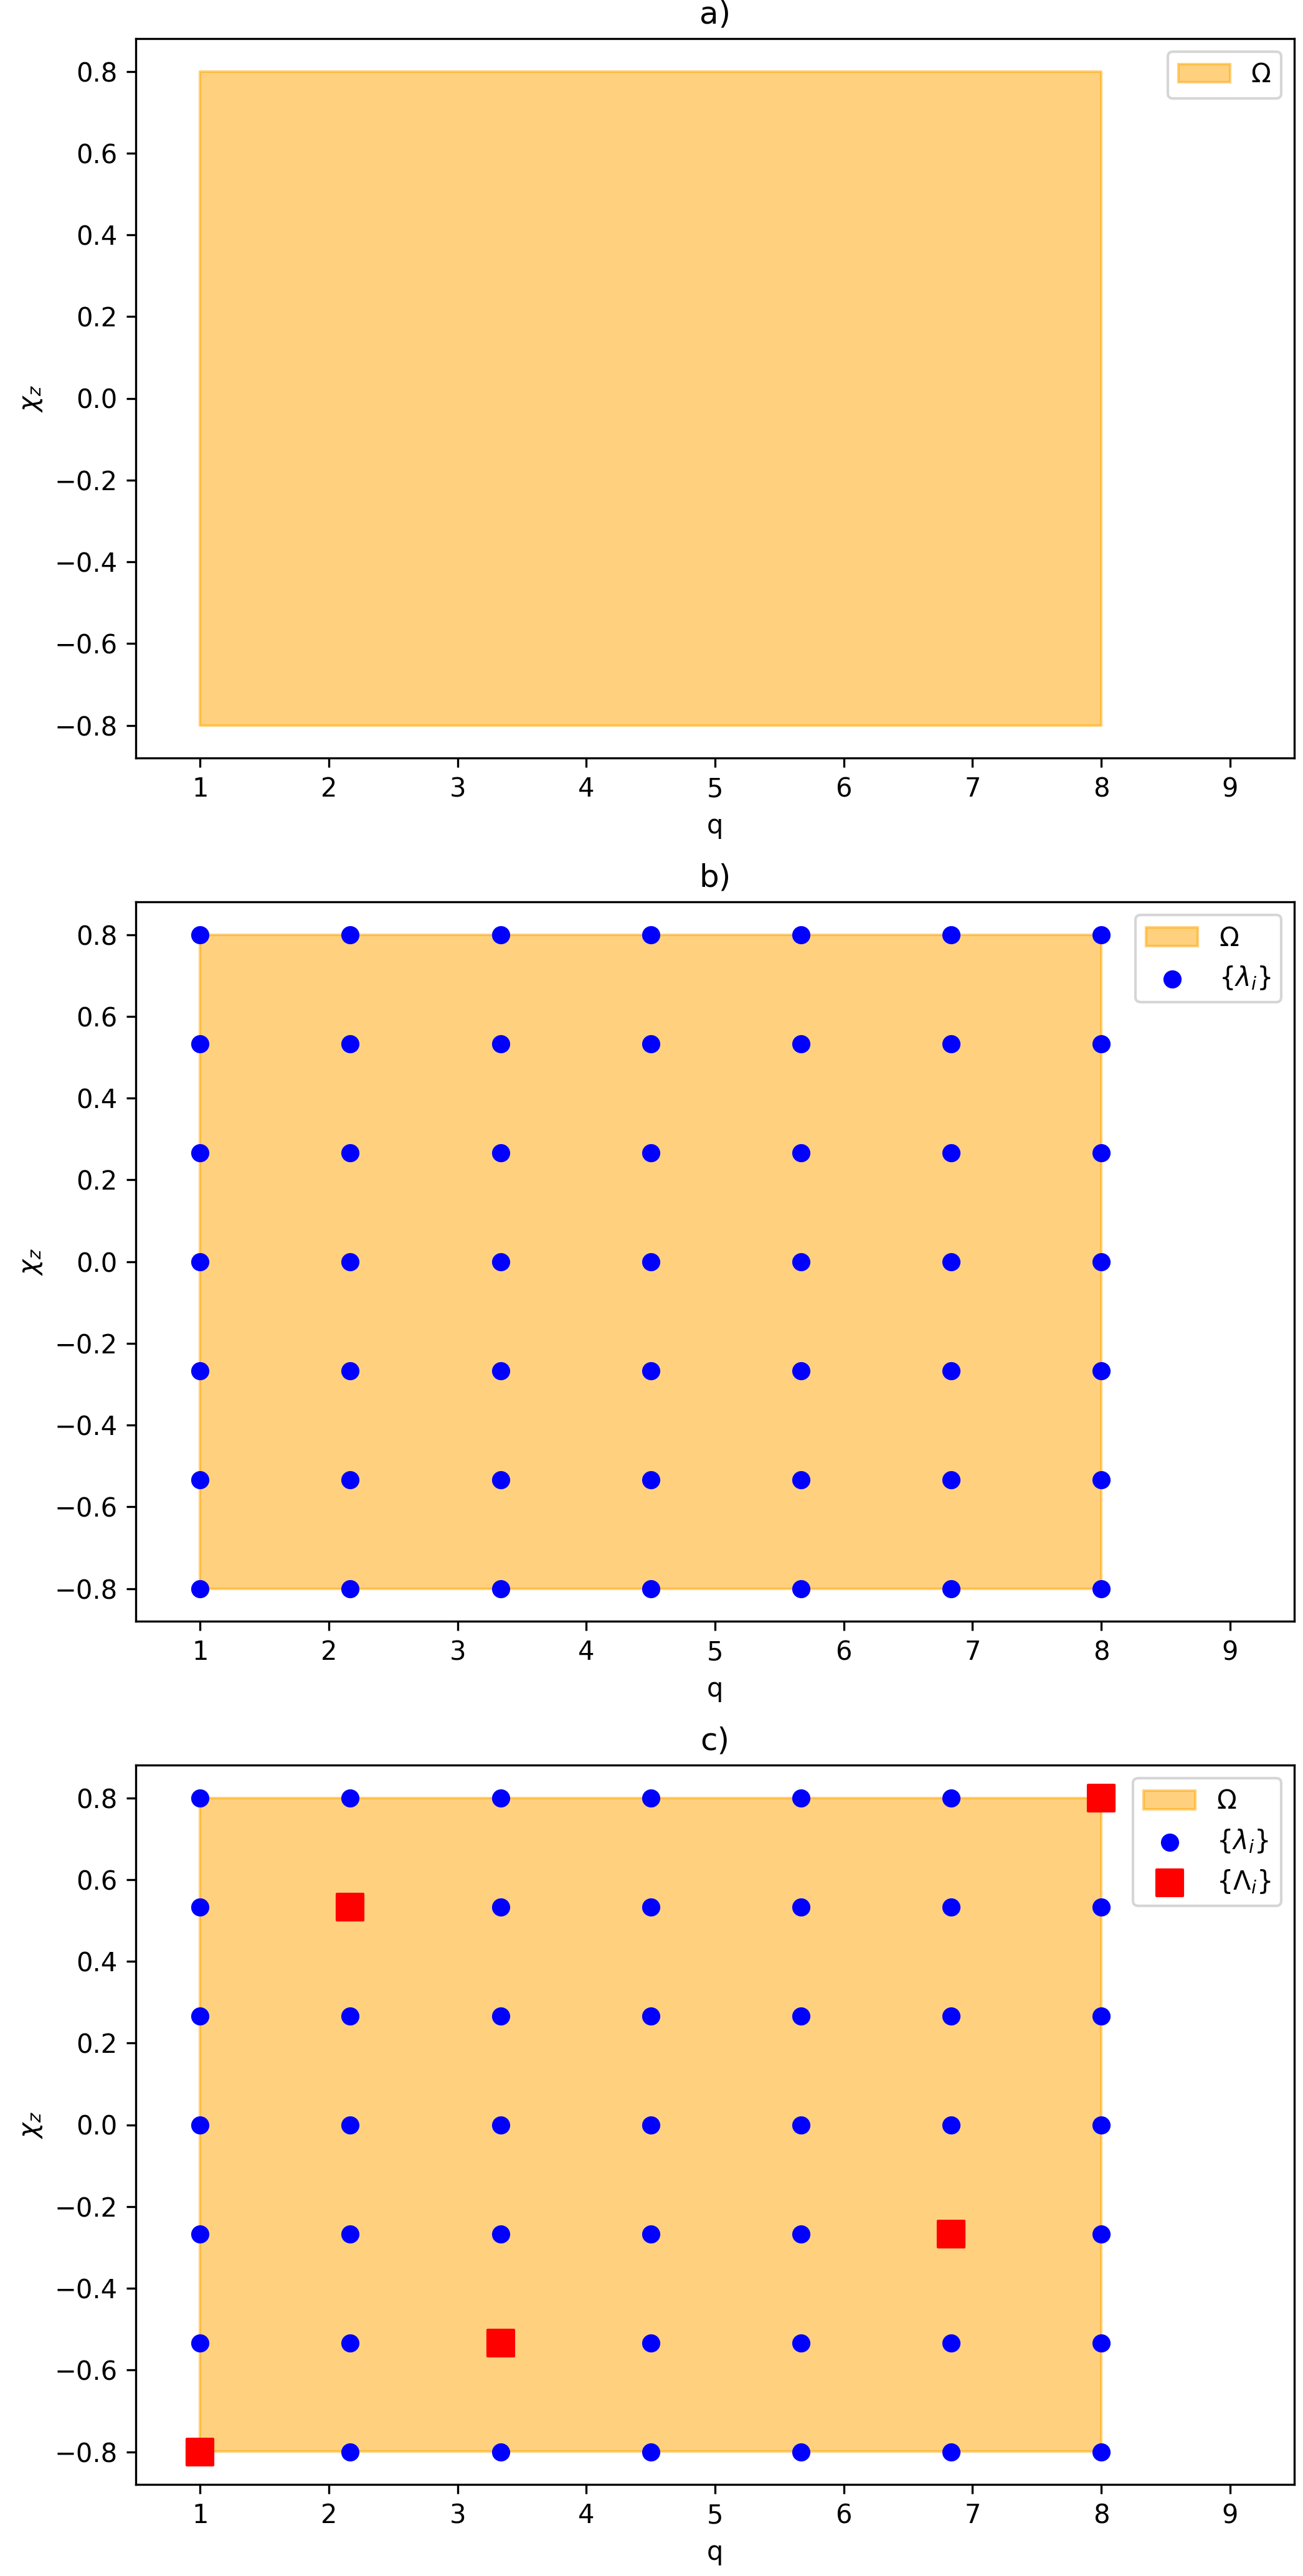
\includegraphics[width=.75\columnwidth]{figs/rb_visual.png}
\caption{a) Representación del espacio $\Omega$. b) Los puntos azules son resultado de un muestro equiespaciado en el espacio $\Omega$, cada punto es un parámetro $\lambda_i$ que representa a una onda $h_{\lambda_i}$. c) Los cuadrados rojos representan a los parámetros \textit{greedy} $\{\Lambda_i\}$, a partir de los cuales se construye la base reducida.}
\label{fig:visual_rb}
\end{figure}

\subsection{Elección de una base óptima}


La pregunta de que tan bien se puede aproximar el espacio $\mathcal{F}$ a partir de una base $\{e_i\}_{i=1}^n$ se puede caracterizar utilizando la definición de la distancia de Kolmogorov \cite{Pinkus1985nWidthsIA}:

\begin{equation} \label{eq:kolmogorov}
d_n := \min_{\{e_i\}_{i=1}^n} \max_{\lambda \in \Omega} \min_{ c_{i,\lambda} \in \mathbb{C}} \| h_{\lambda} - \sum_{i=1}^{n} c_{i,\lambda} e_i(t)\|^2.
\end{equation}



Esta distancia es básicamente es una medida del máximo error de representación en un espacio compacto de parámetros $\Omega$, con una base y coeficientes óptimos.

El producto interno $\|\cdot\|$ en \eqref{eq:kolmogorov} está dado por

\[
\|h_{\lambda}\|^2 :=\int_{t_i}^{t_f}|h_{\lambda}(t)|^2dt
\]
definido a partir del producto interno
\[
\langle h_1, h_2 \rangle  :=\int_{t_i}^{t_f} \overline{h_{1}}(t) h_2 (t)dt
\]

Para entender la notación en $d_n$, se explica el significado de los $\min$, $\max$, $\min$ de derecha a izquierda:

\begin{itemize}
\item $\min_{ c_{i,\lambda} \in \mathbb{C}}$ se refiere a la representación óptima con respecto a la base utilizada. Esto implica realizar una proyección ortogonal a la base. Suponiendo una base ortonormal los coeficientes óptimos serán:

\begin{equation} \label{eq:coefs}
c_{i, \lambda} = \langle e_i, h_{\lambda} \rangle 
\end{equation}

Y se puede reescribir la ecuación \eqref{eq:kolmogorov} de la siguiente forma:
\[
d_n := \min_{\{e_i\}_{i=1}^n} \max_{\lambda \in \Omega} || h_{\lambda} - \mathcal{P}_nh_{\lambda} ||^2.
\]

con 
\begin{equation}
\mathcal{P}_nh_{\lambda} = \sum_{i=1}^{n} c_{i,\lambda} e_i(t)
\end{equation}

\item $\max_{\lambda \in \Omega}$ hace referencia a que se tiene en cuenta el peor error (el máximo) en el espacio de parámetros $\Omega$. 
\item Por último $\min_{\{e_i\}_{i=1}^n}$ implica elegir la base óptima que de lugar al \textit{mejor peor error} en el dominio de parámetros.
\end{itemize}

Por lo tanto $d_n$ sirve como un límite superior; es lo mejor que se puede lograr si la base fue escogida de forma óptima.
En algunos casos $d_n$ se puede calcular teóricamente \cite{MAGARILILYAEV200197}. Más específicamente se puede probar que $d_n \sim n^{-r}$ para funciones con sus primeras $(r-1)$ derivadas continuas y que $d_n \sim e^{-an^b}$ para funciones con una dependencia $C^{\infty}$  \cite{articleg}. En el contexto de ondas gravitacionales se espera un comportamiento asintótico de convergencia exponencial con $n$ \citep{PhysRevX.4.031006, Herrmann:2012xpx}.

La elección de una base óptima es una tarea complicada de complejidad combinatoria y no aplicable en la práctica. Por lo tanto se utilizará un acercamiento más eficiente en base al uso de un algoritmo de tipo voraz o \textit{greedy}, que da lugar a una base cuasi-óptima en un sentido matemático, de complejidad lineal. Para más detalles se recomienda ver \cite{Tiglio:2021ysj}.

\subsection{Algoritmo \textit{Greedy} para construir una base cuasi-óptima}

Un algoritmo de tipo \textit{greedy} es un proceso iterativo en el cual a cada paso se toma la elección que produzca el mayor beneficio inmediato \footnote{Los algoritmos de tipo \textit{greedy} se usan en muchos contextos, y no están asociados únicamente a la construcción de bases reducidas.}.

En el contexto de las bases reducidas, cada iteración del algoritmo agregará a la base el elemento que daba lugar al peor (máximo) error de representación con la base anterior. Es decir que en cada iteración se reducirá el máximo error de representación de todo el conjunto de entrenamiento.


Para cada solución $h_{\lambda}$ del conjunto de entrenamiento, el error de representación es $\| h_{\lambda} - \mathcal{P}_nh_{\lambda} \|^2$, por lo tanto el máximo error de representación o ``Error \textit{greedy}", se define como :

\begin{equation}
\sigma_n := \max_{\lambda \in  \{ \lambda_{i}\}_{i=1}^N } \| h_{\lambda} - \mathcal{P}_nh_{\lambda} \|^2.
\end{equation}

Este error es el \textit{error de entrenamiento}, que disminuirá con cada iteración del algoritmo. También se hablará del \textit{error de validación}, que es el máximo error de representación que ocurre dentro de un conjunto de validación, generalmente más denso que el conjunto de entrenamiento.

El proceso de construcción de una base reducida se puede ver en el algoritmo \ref{alg:rb}, y se explica a continuación:

\begin{itemize}
\item Al algoritmo ingresan tres elementos:
	\begin{itemize}
	\item [--] Un conjunto de entrenamiento $\mathcal{T} = \{ \lambda_{i}, h(\lambda_i) \}_{i=1}^N$ (que incluye tanto las funciones de onda como los parámetros de las funciones), 
	\item[--] El número máximo de elementos permitidos en la base $n_{max}$,
	\item[--] El mínimo error de tolerancia $\varepsilon$ también llamado \textit{tolerancia greedy}.
	\end{itemize}

\item El primer elemento de la base reducida se elije de forma arbitraria a partir del conjunto de parámetros $\{\lambda_{i}\}_{i=1}^N$. El primer parámetro elegido se llama \textit{semilla} o primer parámetro \textit{greedy} $\Lambda_1$. Luego el primer elemento será $h(\Lambda_1)$, pero normalizado.
\item Luego iterativamente se agregan nuevos elementos a la base, seleccionando los parámetros que den lugar al mayor error dentro del conjunto de entrenamiento. El conjunto de estos parámetros recibe el nombre de \textit{parámetros greedy}.
En la figura \ref{fig:visual_rb} c) se observan en color rojo 5 parámetros \textit{greedy}.

\item Por conveniencia a la hora de realizar proyecciones en el espacio generado por la base, se construye una base ortonormal (de forma que los coeficientes $c_{i,\lambda}$ se obtengan por medio de la ecuación \eqref{eq:coefs}). Para esto se aplica un algoritmo de ortonormalización de Gram-Schmidt (líneas 9 y 10 del algoritmo \ref{alg:rb}).
\item El algoritmo finaliza cuando se alcanzó el número máximo de elementos en la base $n = n_{max}$, o cuando el máximo error de representación $\sigma_n$ sea menor al error de tolerancia $\varepsilon$, lo que ocurra primero. El algoritmo devuelve los elementos de la base reducida $\{ e_i\}_{i=1}^{n}$, el conjunto de parámetros \textit{greedy} $\{\Lambda_i\}_{i=1}^{n}$ y el error de representación $\sigma_n$.
\end{itemize}

\begin{algorithm}
\caption{\texttt{GreedyRB}\((\mathcal{T}, \varepsilon, n_{max})\)}\label{alg:rb}
\begin{algorithmic}[1]
\Require $\mathcal{T} = \{ \lambda_{i}, h(\lambda_i) \}_{i=1}^N, \varepsilon, n_{max}$ 
\vspace{3mm}
\State $i = 1$
\State $\sigma_1 = 1$ \Comment{Inicializar error de representación a 1}
\State $\Lambda_1 = \lambda_k$	\Comment{Elección arbitraria de la semilla}
\State $e_1 = h(\Lambda_1)/||h(\Lambda_1)||$	
\State $\text{rb}=\{e_1\}$	\Comment{Primer elemento de la base reducida}
\vspace{2mm}
\While{$\sigma_i > \varepsilon$ \textbf{and} $i < n_{max}$}
	\State $i = i+1$
	\State $\Lambda_i = 	arg \max_{\lambda \in \mathcal{T}}||h_{\lambda}-\mathcal{P}_{i-1}h_{\lambda}||^2$ \Comment{Selección del parámetro \textit{greedy}}
	\State $e_i = h(\Lambda_i) - {P}_{i-1}h(\Lambda_i)$ \Comment{Gram-Schmidt}
	\State $e_i = e_i / ||e_i|| $ \Comment{Normalización}	
	\State $\text{rb} = \text{rb} \cup \{e_i\}$
	\State $\sigma_i = \max_{\lambda \in \mathcal{T}}||h_{\lambda}-\mathcal{P}_{i}h_{\lambda}||^2$	\Comment{Error de representación}
\EndWhile
\vspace{3mm}
\Ensure $\text{rb} = \{ e_i\}_{i=1}^{n},\Lambda = \{\Lambda_i\}_{i=1}^{n}, \sigma_n$
\end{algorithmic}
\end{algorithm}


\subsection{Convergencia del Algoritmo \textit{Greedy}}

Para una tolerancia \textit{greedy} $\varepsilon$ el algoritmo \textit{greedy} entrega una base reducida con un error

\[
\sigma_n = \max_{\lambda \in  \{ \lambda_{i}\}_{i=1}^N } || h_{\lambda} - \mathcal{P}_nh_{\lambda} ||^2 \leq \varepsilon
\]

Dado que la elección del primer elemento de la base reducida es arbitrario (la elección de la semilla), el lector o lectora podría preguntarse que tan relevante es esta elección a la hora de condicionar la convergencia del error de representación $\sigma_n$.
Como se mencionó anteriormente, la medida de Kolmogorov $d_n$ puede utilizarse como cota superior. 
Resultados obtenidos en \cite{https://doi.org/10.48550/arxiv.1204.2290} muestran que si $d_n$ decae exponencialmente, $\sigma_n$ también lo hará:

\[
d_n \leq De^{-an^{\alpha}} \ \ \rightarrow \ \ \sigma_n \leq \sqrt{2D} \gamma^{-1} e^{-a_{\alpha}'n^{\alpha}},
\]
con $D$, $\alpha$, $a$ constantes positivas y $\gamma \in (0,1]$.
De forma similar, si el decaimiento de $d_n$ es polinomial, también lo será el decaimiento de $\sigma_n$:
\[
d_n \leq D n^{-\alpha} \ \ \rightarrow \ \ \sigma_n \leq D_{\alpha}'n^{-\alpha},
\]
con $D$, $\alpha > 0$ y $\gamma \in (0, 1]$.

En la Figura \ref{fig:rb_vs_n} se puede ver el decaimiento exponencial del error de representación en función del número de elementos de la base reducida aplicado en el contexto de ondas gravitacionales \cite{Caudill_2012}. Lo más relevante es que se puede ver que este comportamiento no depende de la elección de la raíz. El área sombreada representa los extremos de todas las posibles semillas dentro del conjunto de entrenamiento.


\begin{figure}[h!]
\centering
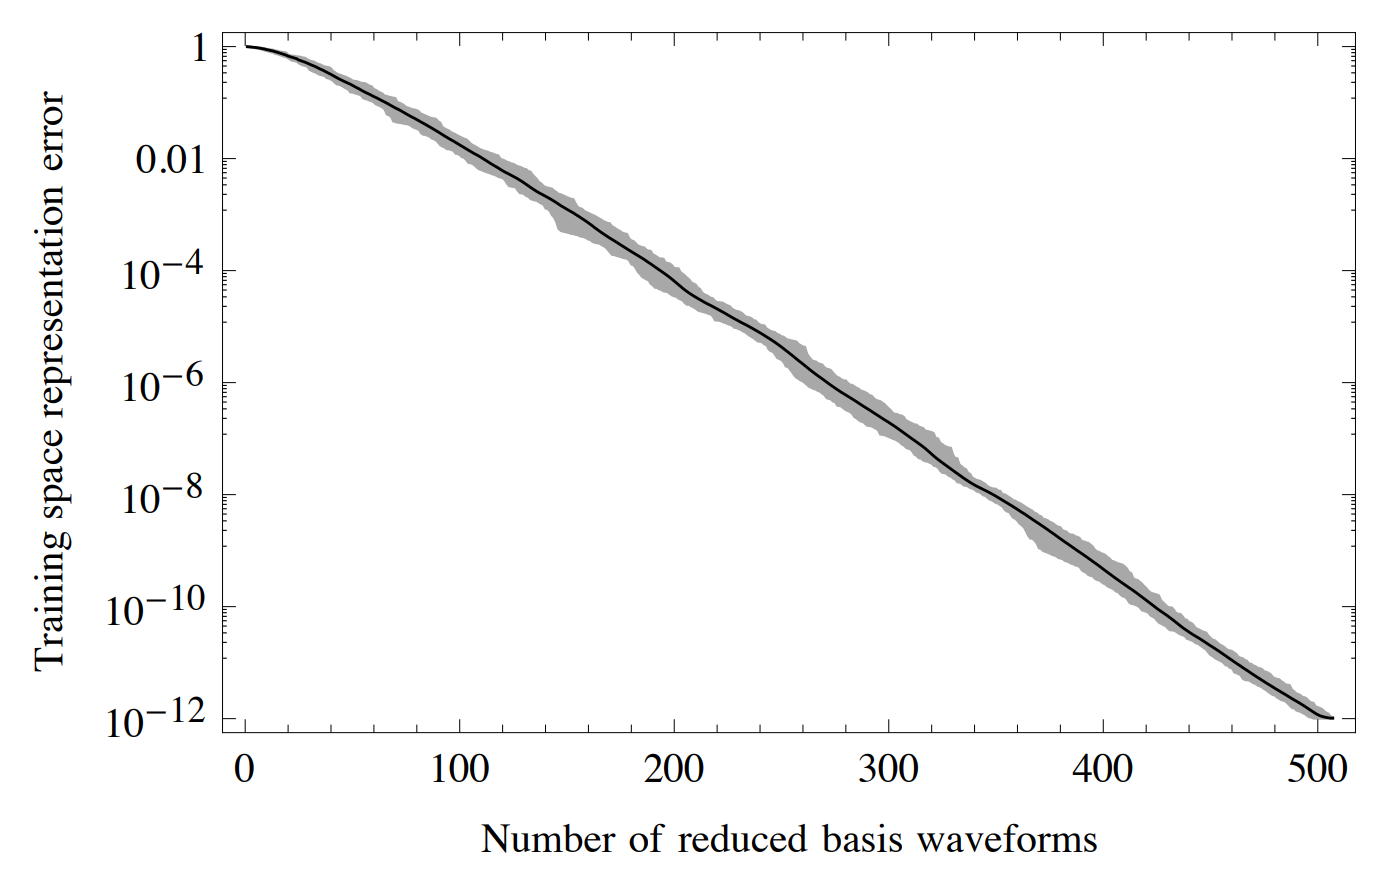
\includegraphics[width=.8\columnwidth]{figs/rb_vs_n.png}
\caption{Error de representación en función del número de funciones de onda en la base reducida para un modo cuasinormal (QNM). Se probaron todas las semillas posibles del conjunto de entrenamiento; en negrita se ve el promedio, y el área sombreada representa los valores extremos \cite{Caudill_2012}.}
\label{fig:rb_vs_n}
\end{figure}

\section{Bases Reducidas hp Greedy}

El nombre del método \textit{hp-greedy} \cite{Cerino:2022dhr} surge de la combinación del \textit{``refinamiento p''} y del \textit{``refinamiento h"}. El \textit{refinamiento p} proviene de los métodos espectrales con bases polinomiales \cite{hesthaven_gottlieb_gottlieb_2007} y se refiere a la propiedad de que el error de representación disminuye al aumentar el grado del polinomio (en el caso de las bases reducidas aumenta el número de elementos en la base). Por otro lado el término de \textit{refinamiento h} se toma prestado de los métodos de diferencias finitas, donde el tamaño de cada celda de la grilla es representado por \textit{h}, y este se refina para obtener un mejor resultado. En el caso de las bases reducidas \textit{hp-greedy} este último refinamiento ocurre en el espacio de los parámetros y no en el dominio físico.

\subsection{Refinamiento h}

Partiendo de la siguiente notación:
\begin{itemize}
\item $V$: espacio de parámetros para un dado subdominio.
\item $\Omega$: espacio total de parámetros tal que $\Omega= \cup V$.
\item $V_1, V_2$ : particiones de $V$.
\item $\Lambda_V$ : parámetros \textit{greedy} en $V$.
\item  $\hat{\Lambda}_{V}$: punto de anclaje para $V$.
%\item  $\hat{\Lambda}_{V_1}, \hat{\Lambda}_{V_2}$
\end{itemize}

El refinamiento en el dominio de los parámetros ocurre a partir de la división recursiva de cada subdominio $V \subseteq \Omega$ en dos subdominios $V_1$ y $V_2$. La división de cada dominio $V$ se realizará en función de dos puntos de anclaje $\hat{\Lambda}_{V_1}$ y $\hat{\Lambda}_{V_2}$. Estos puntos de anclaje no son más que los primeros dos elementos del conjunto de parámetros \textit{greedy} $\Lambda_V$.
Como resultado de estas divisiones iterativas se obtiene una estructura de árbol binario.


Esta descomposición binaria del dominio está descrita en forma de pseudocódigo en el algoritmo \ref{alg:part}.

Al algoritmo ingresan tres objetos:

\begin{itemize}
\item $\lambda_V$: conjunto de parámetros resultado de un muestreo de $V$.
\item $\hat{\Lambda}_{V_1}, \hat{\Lambda}_{V_2}$: puntos de anclaje (son los primeros dos elementos de $\Lambda_V$).
\end{itemize}

Luego, para cada parámetro del conjunto $\lambda_V$ se evalúa su distancia a los puntos de anclaje a partir de la \textit{función de proximidad} $d: d(\lambda_1, \lambda_2)$:

\[
d(\lambda_1, \lambda_2) = ||\lambda_1 - \lambda_2||_2,
\]

de forma que se obtengan dos conjuntos; $\lambda_{V_1}$ con los $\lambda_{i}$ más próximos a $\hat{\Lambda}_{V_1}$, y $\lambda_{V_2}$ con los $\lambda_{i}$ más próximos a $\hat{\Lambda}_{V_2}$, tal que  $\lambda_{V} =\lambda_{V_1} \cup \lambda_{V_2}$. Este resultado es la división del espacio de parámetros a partir de los puntos de anclaje.

\begin{algorithm}
\caption{\texttt{Partition}\((\lambda_V, \hat{\Lambda}_{V_1}, \hat{\Lambda}_{V_2})\)}\label{alg:part}
\begin{algorithmic}[1]
\Require $\lambda_V, \hat{\Lambda}_{V_1}, \hat{\Lambda}_{V_2}$ 
\vspace{3mm}
\State $\lambda_{V_1} = \lambda_{V_2} = \emptyset$
\For{\textbf{each} $\lambda_i \in \lambda_V$}
	\If{$d(\lambda_i, \hat{\Lambda}_{V_1}) <d(\lambda_i, \hat{\Lambda}_{V_2})$}
		\State $\lambda_{V_1} = \lambda_{V_1} \cup \lambda_i$
	\ElsIf{$d(\lambda_i, \hat{\Lambda}_{V_1}) >d(\lambda_i, \hat{\Lambda}_{V_2})$}
		\State $\lambda_{V_2} = \lambda_{V_2} \cup \lambda_i$
	\Else
		\State $\lambda_{V'} = $ random choice$([\lambda_{V_1}, \lambda_{V_2}])$
		\State $\lambda_{V'} = \lambda_{V'} \cup \lambda_i$
	\EndIf
\EndFor
\vspace{3mm}
\Ensure $\lambda_{V_1}, \lambda_{V_2}$
\end{algorithmic}
\end{algorithm}

\subsection{Refinamiento hp-greedy}


El refinamiento \textit{hp-greedy} es un método que combina el algoritmo greedy para la construcción de bases reducidas con la partición del dominio de parámetros. 

Esta partición recursiva del dominio de parámetros da lugar a una estructura de árbol binario, la cual tendrá diferentes niveles $l$ de profundidad, con un $l_{max}$ establecido por el usuario, de forma que $l : 0 \le l \le l_{max}$, donde $l =0$ es el nodo raíz. Cada nodo del árbol estará etiquetado por un conjunto de índices $B_l$, que parte de:

\[
B_0 = (0,),
\]
luego sus dos hijos ($l=1$) tendrán las etiquetas:
\[
B_1 = (0,0,) \ \ o \ \  (0, 1, ),
\]
y en general:
\[
B_l = (0, i_1, \cdots, i_l), \ \  con \ \ i_j = \{0, 1\},
\]

\noindent donde cada nivel $l$ tendrá un máximo de $2^l$ nodos.
Los nodos que no tengan hijos se llamarán nodos \textit{hojas}.
\begin{figure}[h!]
\centering
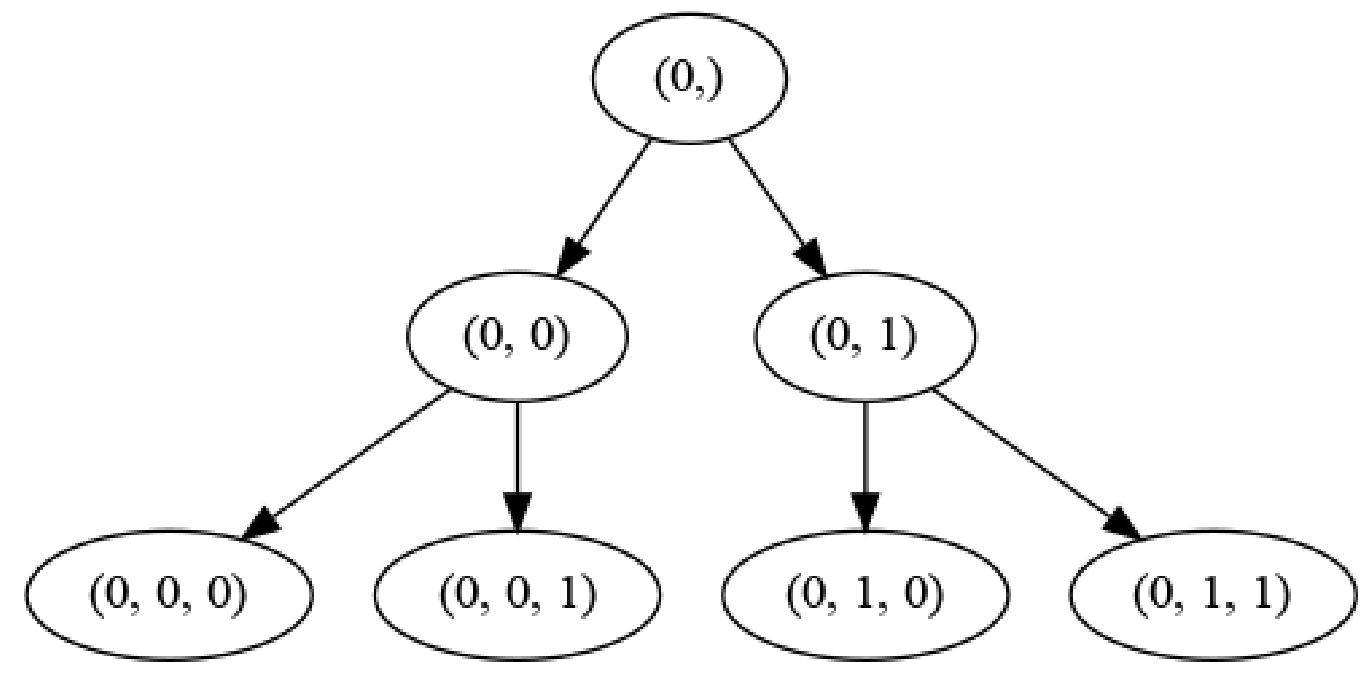
\includegraphics[width=.5\columnwidth]{Bl_lmax2.png}
\caption{Representación de los nodos de un árbol con $l_{max}=2$ \cite{Cerino:2022dhr}.}
\end{figure}

El método está explicado en el algoritmo \ref{alg:hp}; partiendo de un dado dominio de parámetros $V$ se construye una base reducida a partir de un conjunto de entrenamiento $\mathcal{T}_V = \{\lambda_{V_i}, h_{\lambda_{V_i}}\}_{i=1}^{N}$, una \textit{tolerancia greedy} $\varepsilon$ y un $n_{max}$ (para esto se utiliza el algoritmo \ref{alg:rb}). Si el error de representación $\sigma$ es mayor que la tolerancia $\varepsilon$, y si la profundidad del nivel $l$ es menor a $l_{max}$, entonces se realizará una partición del dominio $V$ utilizando como puntos de anclaje a los dos primeros parámetros \textit{greedy}. En cada dominio se realizará el mismo procedimiento hasta que se cumpla que $l = l_{max}$ o hasta que $\sigma \le \varepsilon$.

 % El conjunto $\lambda_V$ representa el conjunto de parámetros de $\mathcal{T}_V$

\begin{algorithm}
\caption{\texttt{hpGreedy}\((\mathcal{T}, \varepsilon, n_{max}, l, l_{max}, B_{l})\)}\label{alg:hp}
\begin{algorithmic}[1]
\Require $\mathcal{T} = \{ \lambda_{i}, h_{i} \}_{i=0}^N, \varepsilon, n_{max},l, l_{max}, B_{l}$ 
\vspace{3mm}
\State rb, $\Lambda_V$, $\sigma$ = \texttt{GreedyRB}($\mathcal{T}_V,\lambda_V, \varepsilon, n_{max}$) 
\vspace{3mm}
\If{$\sigma > \varepsilon$ \textbf{and} $l<l_{max}$}
	\State $\hat{\Lambda}_{V_1} = \Lambda_V[1]$
	\State $\hat{\Lambda}_{V_2} = \Lambda_V[2]$
	\State $\lambda_{V_1}, \lambda_{V_2} =$ \texttt{Partition}$(\lambda_V,\hat{\Lambda}_{V_1}, \hat{\Lambda}_{V_2})$
	\State $out_1 = $ \texttt{hpGreedy}\((\mathcal{T}_{V_1}, \lambda_{V_1}, \varepsilon, n_{max}, l+1, l_{max}, (B_{l}, 0))\)
	\State $out_2 = $ \texttt{hpGreedy}\((\mathcal{T}_{V_2} ,\lambda_{V_2}, \varepsilon, n_{max}, l+1, l_{max}, (B_{l}, 1))\)
	\State $out = out_1 \cup out_2$
\Else
	\State $out = \{( rb, \Lambda_V, B_l)\}$
\EndIf
\vspace{3mm}
\Ensure out
\end{algorithmic}
\end{algorithm}

El resultado del algoritmo \ref{alg:hp} es una estructura arbórea, donde cada nodo contiene la información de sus puntos de anclaje, por lo que en el caso de querer proyectar un conjunto de validación, cada onda gravitacional se proyectará a la base reducida del nodo hoja con el punto de anclaje más cercano al parámetro de la onda. En la figura \ref{fig:part_1d} se puede ver un esquema de la división de parámetros para el caso de un $\lambda$ de una sola dimensión. Luego en la figura \ref{fig:proy_1d} se esquematiza el proceso de proyección de una función $h_{\lambda_i}$ a la base creada.

\begin{figure}[h!]
\centering
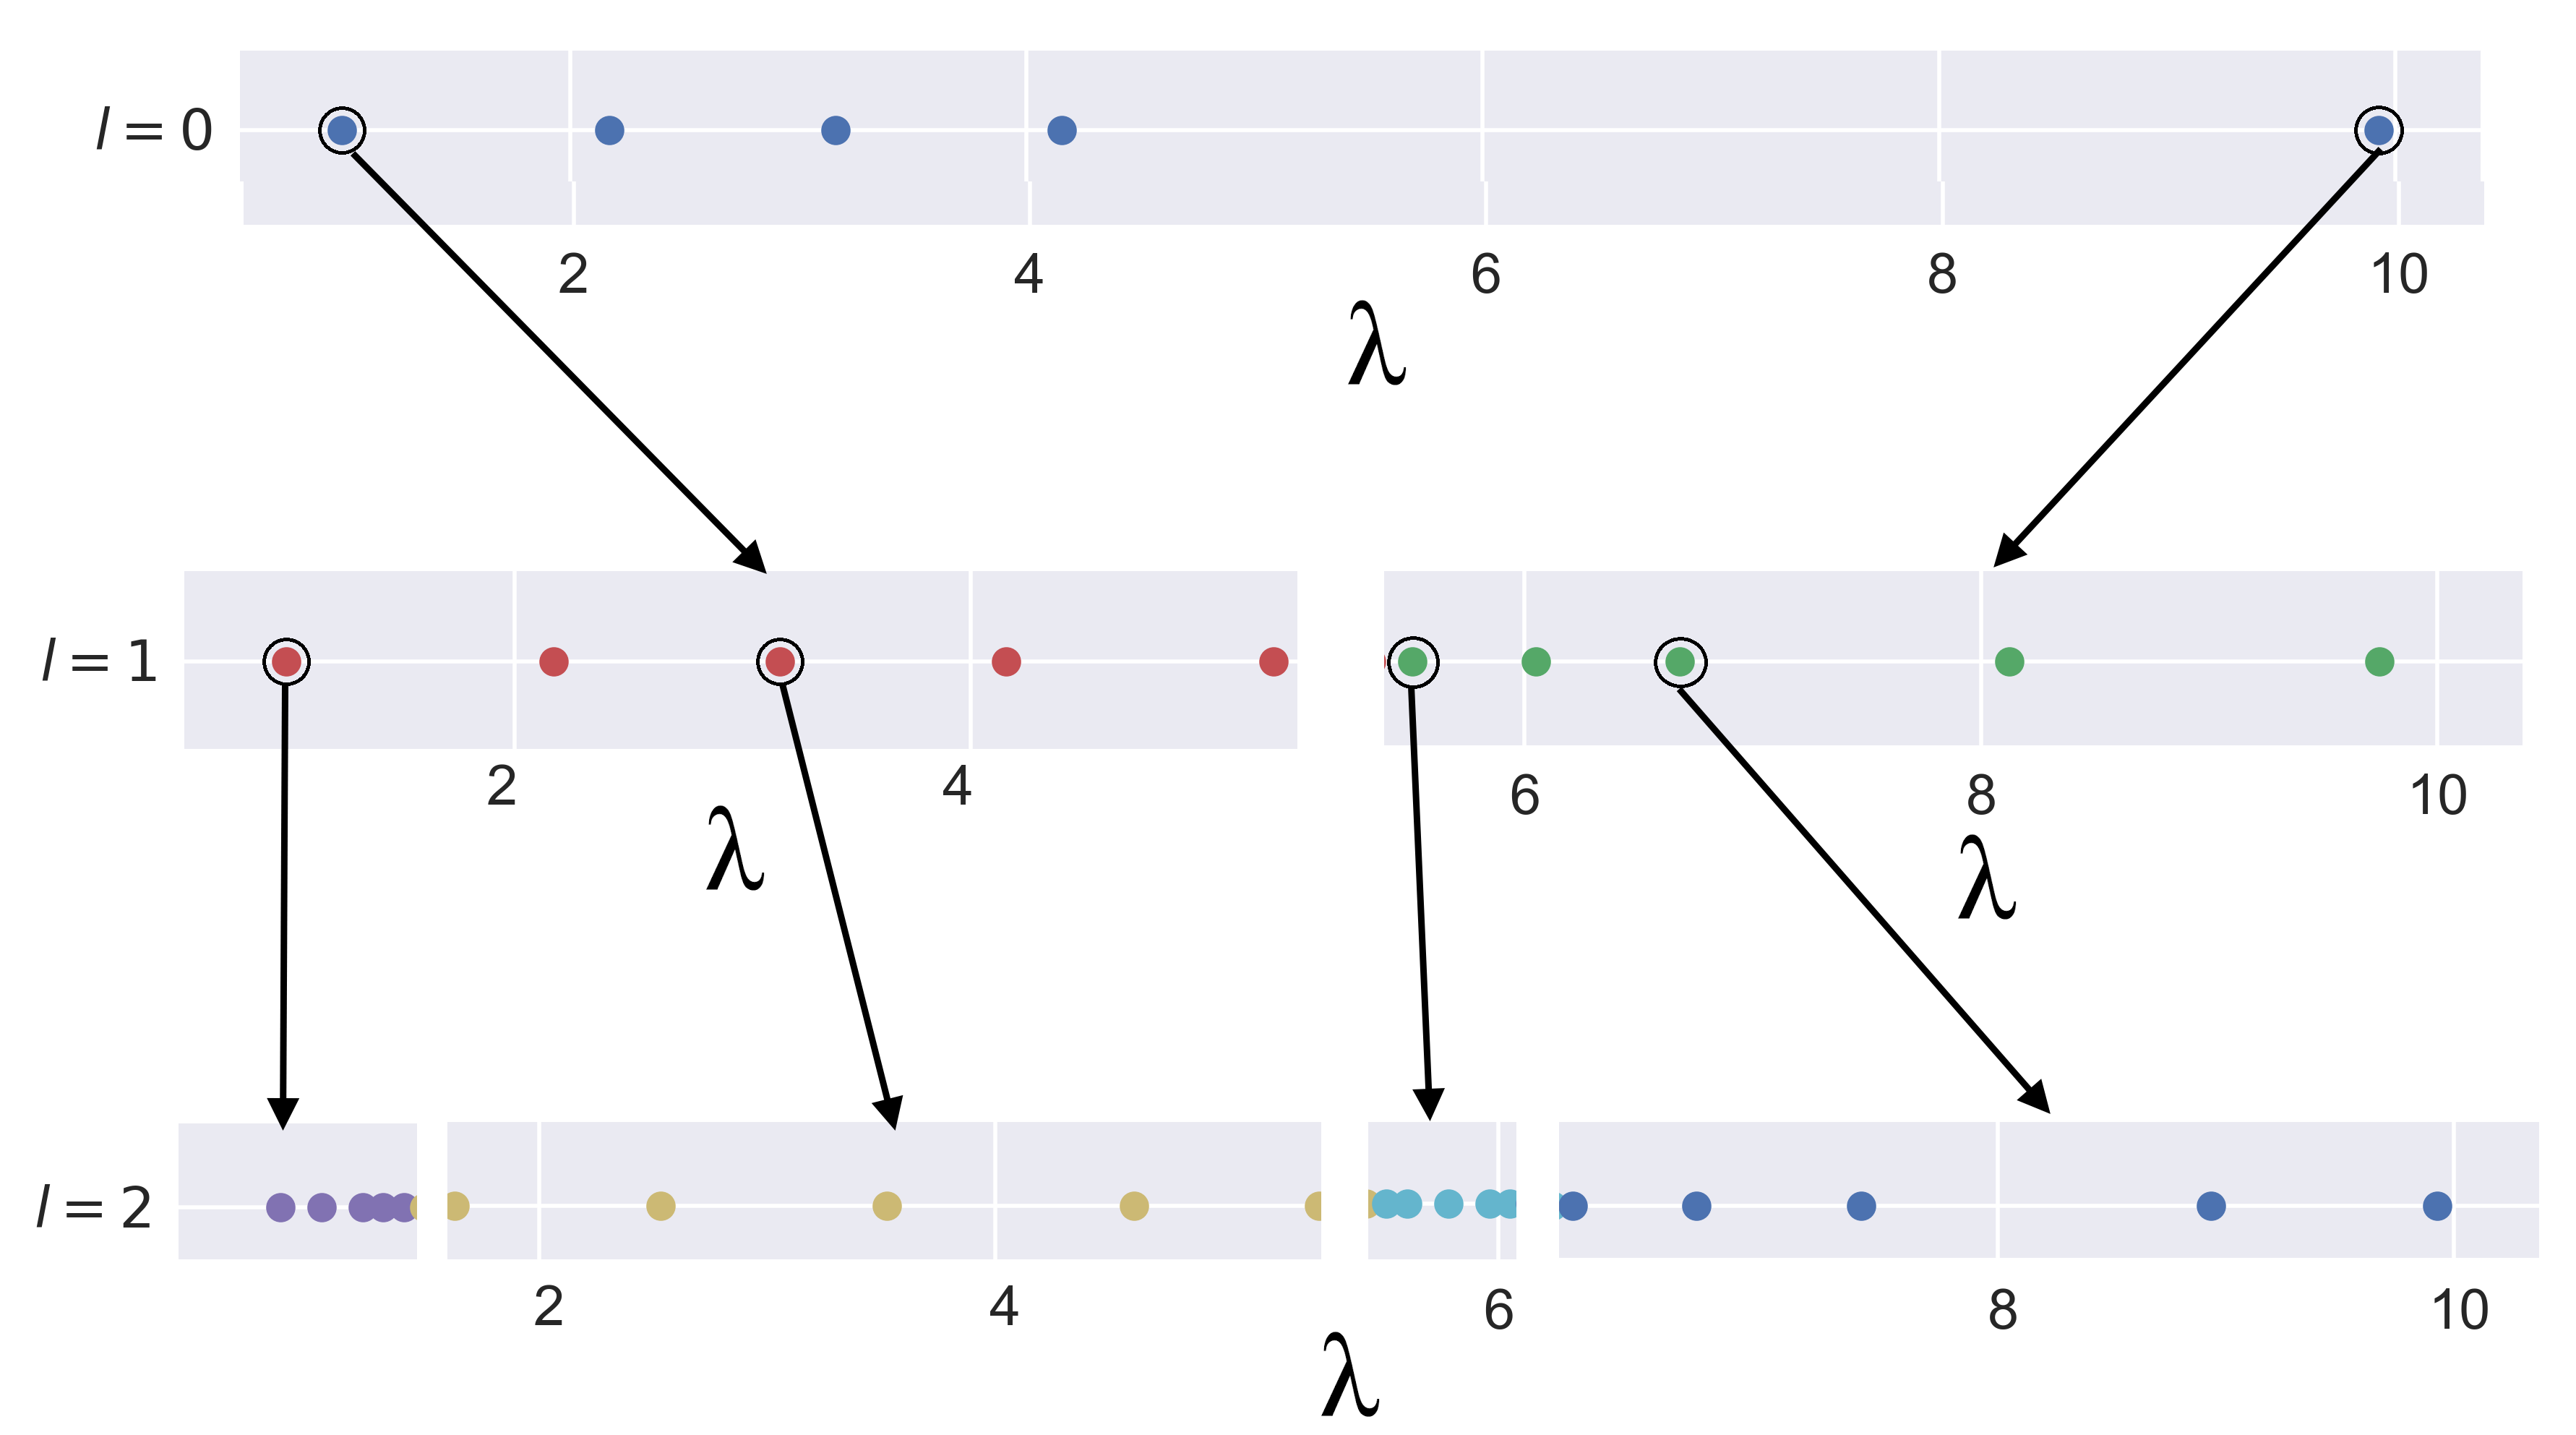
\includegraphics[width=0.75\columnwidth]{figs/particion_parametros_1d.png}
\caption{Ejemplo de partición del dominio de parametros para un parámetro $\lambda$ unidimensional. Los puntos de colores representan a los parámetros \textit{greedy} $\Lambda_V$ para cada subdominio $V$, resaltando a los puntos de anclaje $\Lambda_V$ con un círculo externo. Este diagrama muestra como se divide cada subdominio en función de sus puntos de anclaje. En este ejemplo $n_{max} = 5$ y $l_{max}=2$.}
\label{fig:part_1d}
\end{figure}

\subsection{Tiempo de Proyección}


Un aspecto muy importante del refinamiento \textit{hp-greedy}, que se mencionará seguido de ahora en adelante, es el tiempo de proyección a la base. 


\begin{figure}[h!]
\centering
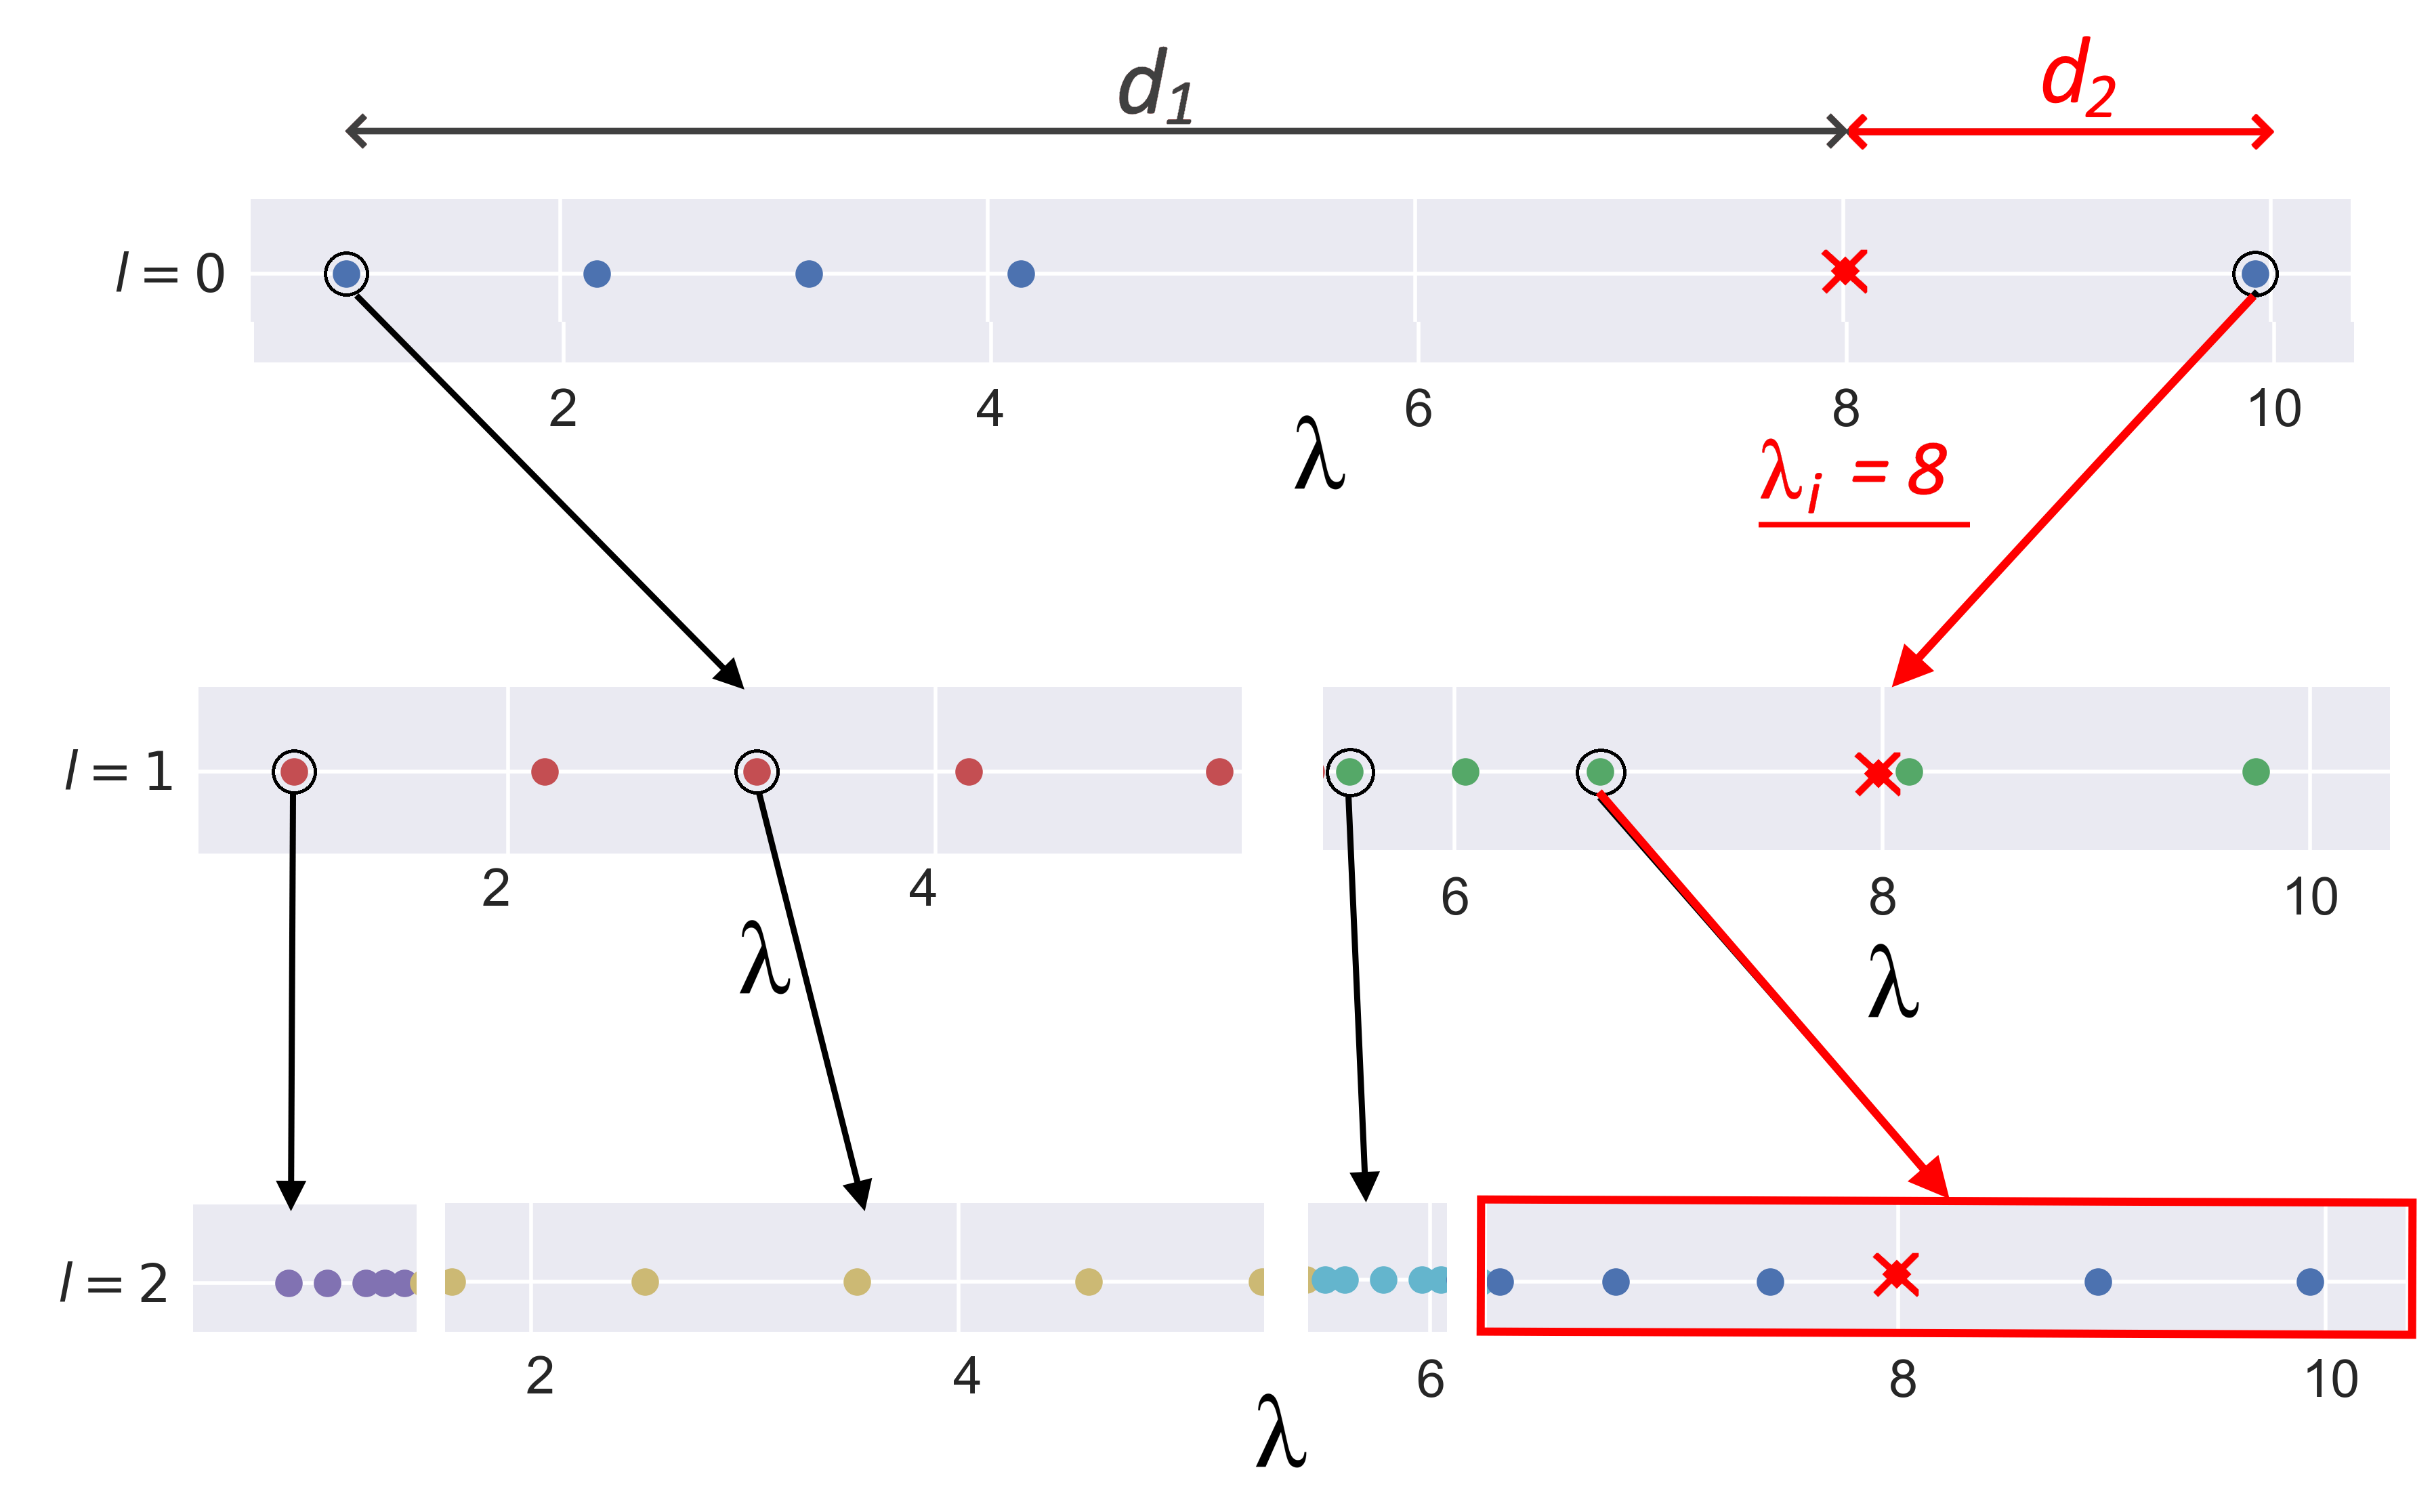
\includegraphics[width=0.75\columnwidth]{figs/proyeccion_1d.png}
\caption{Proyección de una onda $h_{\lambda_i}$ sobre la base de ejemplo de la figura \ref{fig:part_1d} (en este caso $\lambda_i = 8$, marcado con una cruz roja). Partiendo de la raíz del árbol, se calcula iterativamente la distancia entre $\lambda_i$ y los puntos de anclaje de cada subdominio, hasta llegar a alguna de las hojas del árbol. El camino seguido se marca en color rojo.}
\label{fig:proy_1d}
\end{figure}

Al momento de proyectar una función $h_{\lambda_i}$ a una base \textit{hp-greedy}, primero se debe obtener la base local del nodo hoja (ver fig. \ref{fig:proy_1d}) y luego se realiza la proyección a la base encontrada.
Proyectar un conjunto de validación implica repetir este mismo proceso para todas las funciones del conjunto. Este proceso se realizará a lo largo de un tiempo $t$, que se denomina \textit{tiempo de proyección}. 

En el siguiente apartado se analiza el tiempo de proyección en diferentes bases \textit{hp-greedy} en el contexto de ondas gravitacionales.


\subsection{Aplicación a Ondas Gravitacionales}
\label{sec:hp-gw}

En esta subsección se utiliza un conjunto de ondas gravitacionales con parámetro bidimensional $\lambda = (q, \chi_z)$, donde $\chi_{1_z} = \chi_{2_z} = \chi_z$ es el espín de los agujeros negros y $q$ es la relación entre sus masas. De esta forma se puede graficar fácilmente el dominio de parámetros.



En la Figura \ref{fig:part1} se puede observar una representación de la partición del dominio de parámetros. En la primera imagen se pueden ver los dos puntos de anclaje, que son los primeros dos elementos de la base global construida inicialmente. En cada nueva división se construye una nueva base global con la cual se realiza la siguiente partición de cada subdominio.


\begin{figure}[h!]
\centering
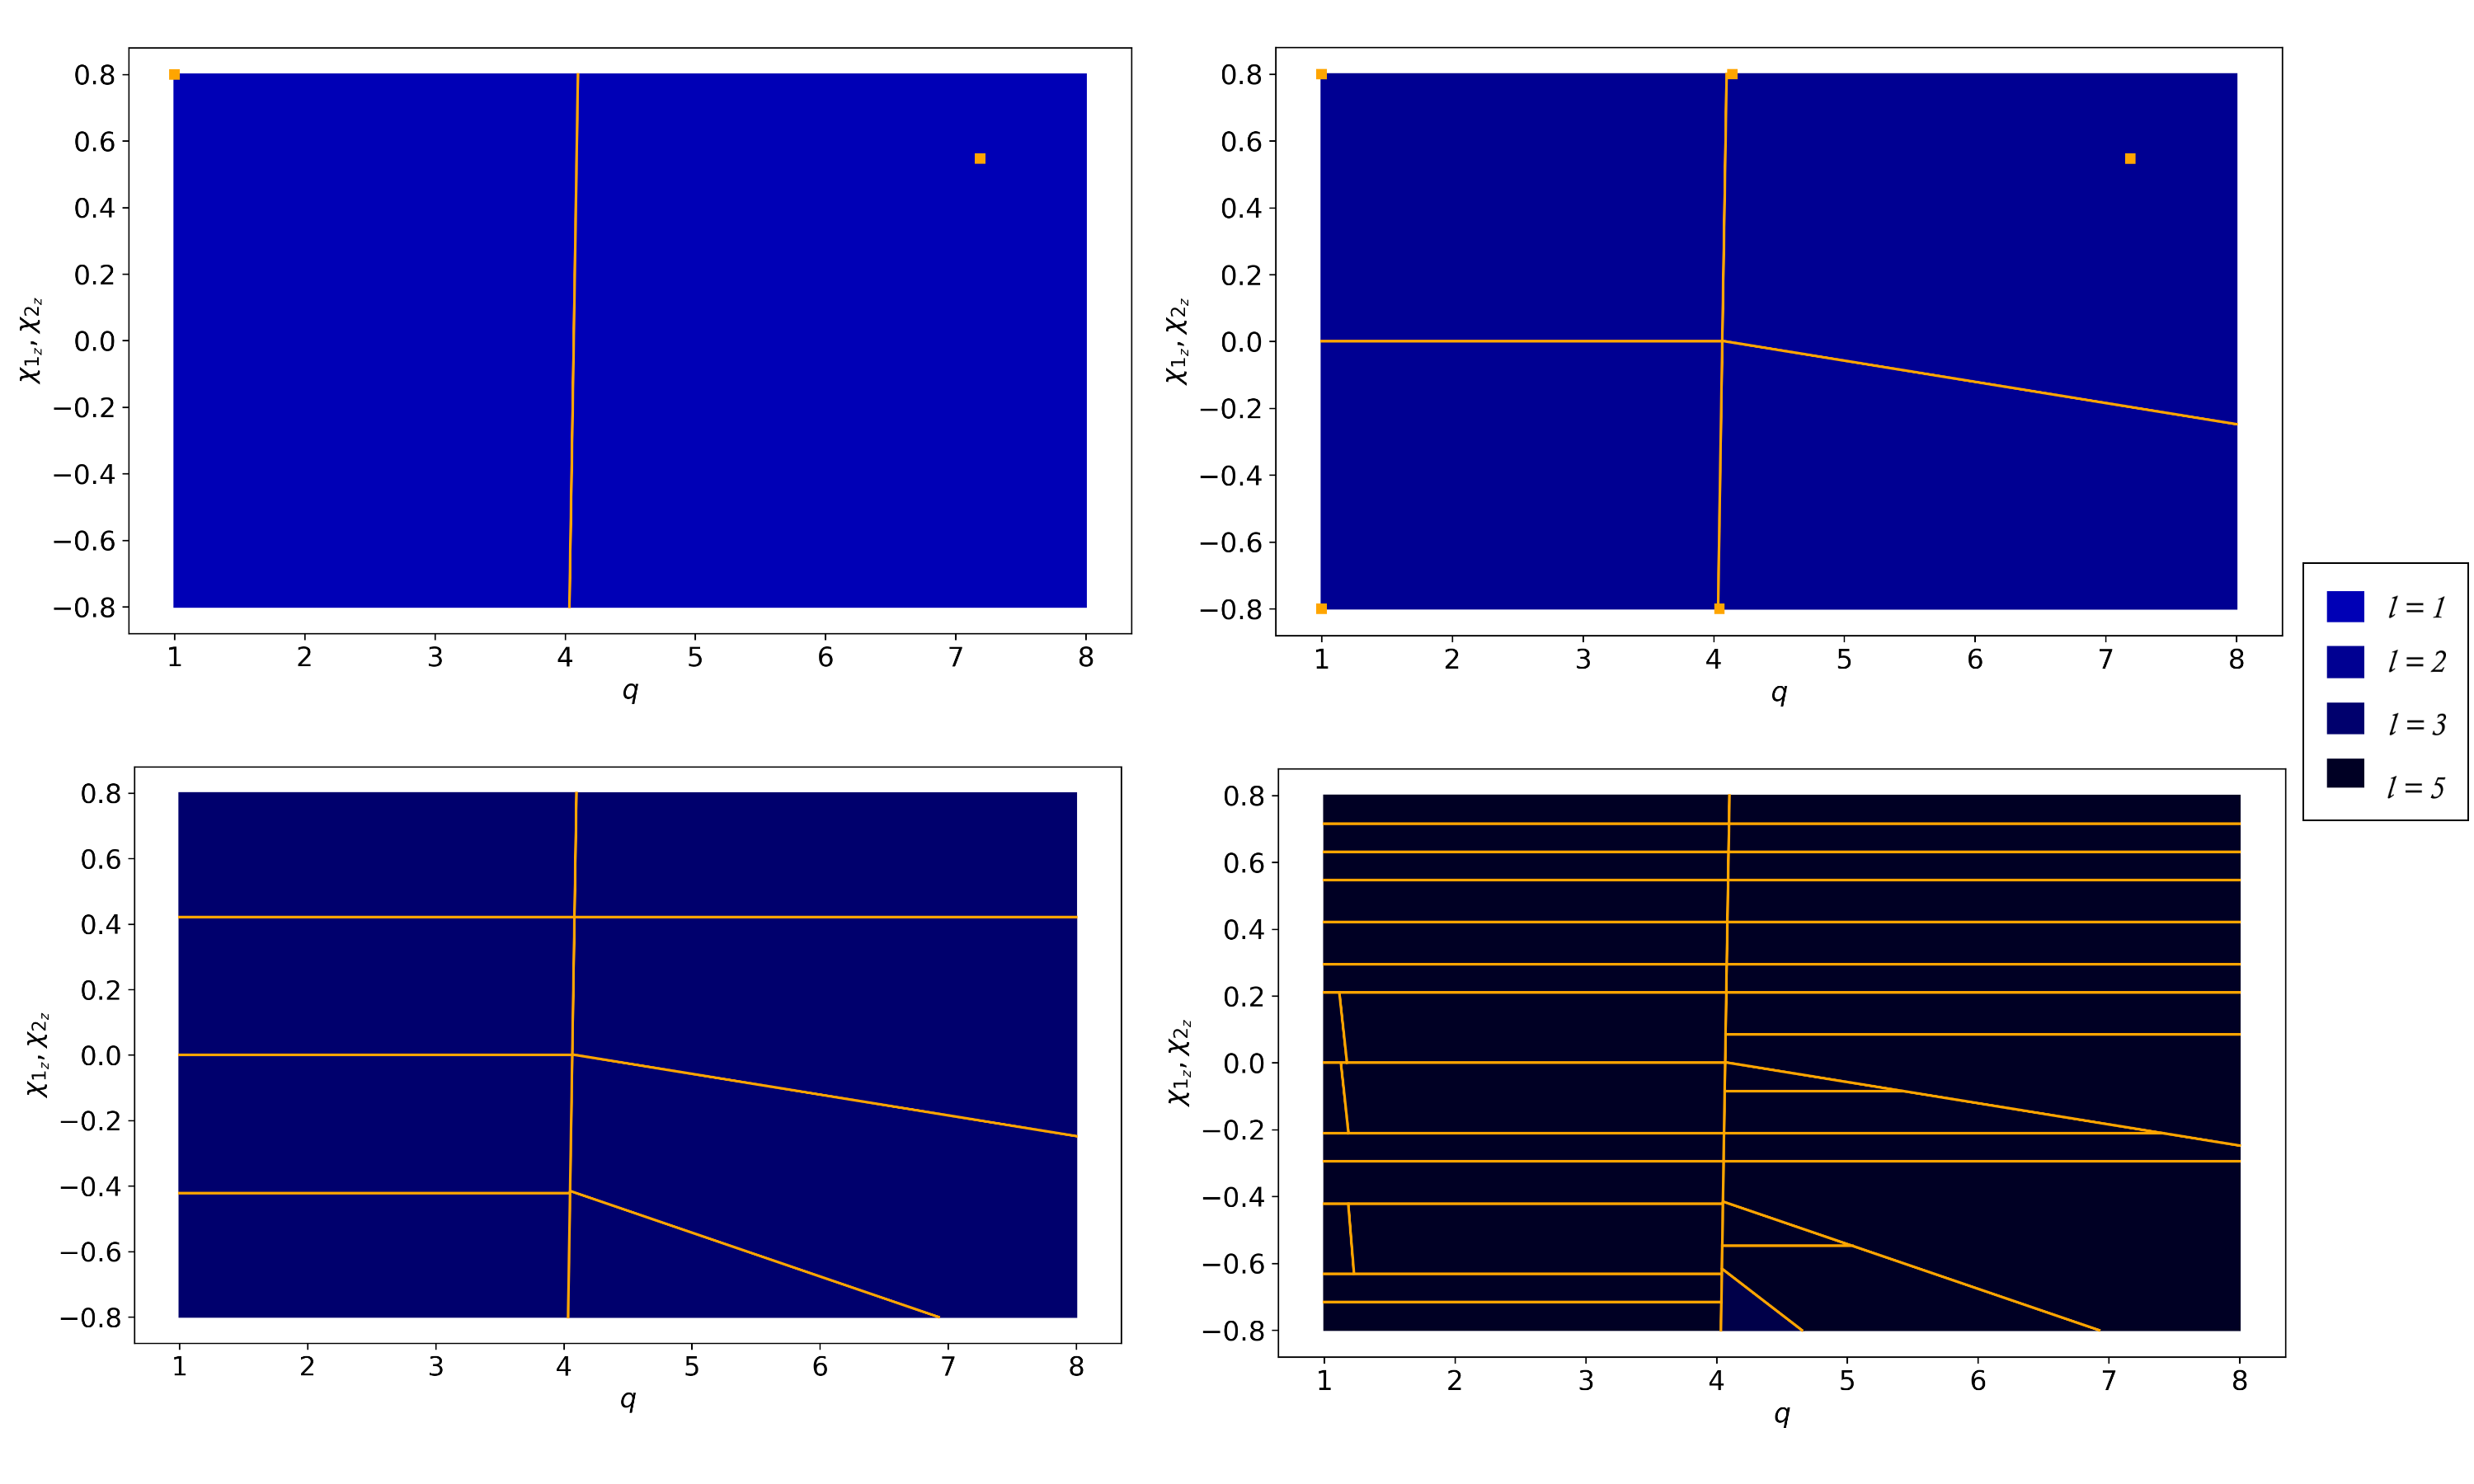
\includegraphics[width=1\columnwidth]{figs/particion2d.png}
\caption{Ejemplo de partición del espacio de parámetros bidimensional para $l_{max}= 1, 2, 3$ y $5$. En los primeros dos casos se muestran los puntos de anclaje en naranja.}
\label{fig:part1}
\end{figure}


En la Figura \ref{fig:l0vl4} se compara el máximo error de representación obtenido para un conjunto de validación con una base global, es decir, con $l_{max} = 0$, y con $l_{max}=4$. La velocidad de convergencia es claramente mayor en el segundo caso.

\begin{figure}[h!]
\centering
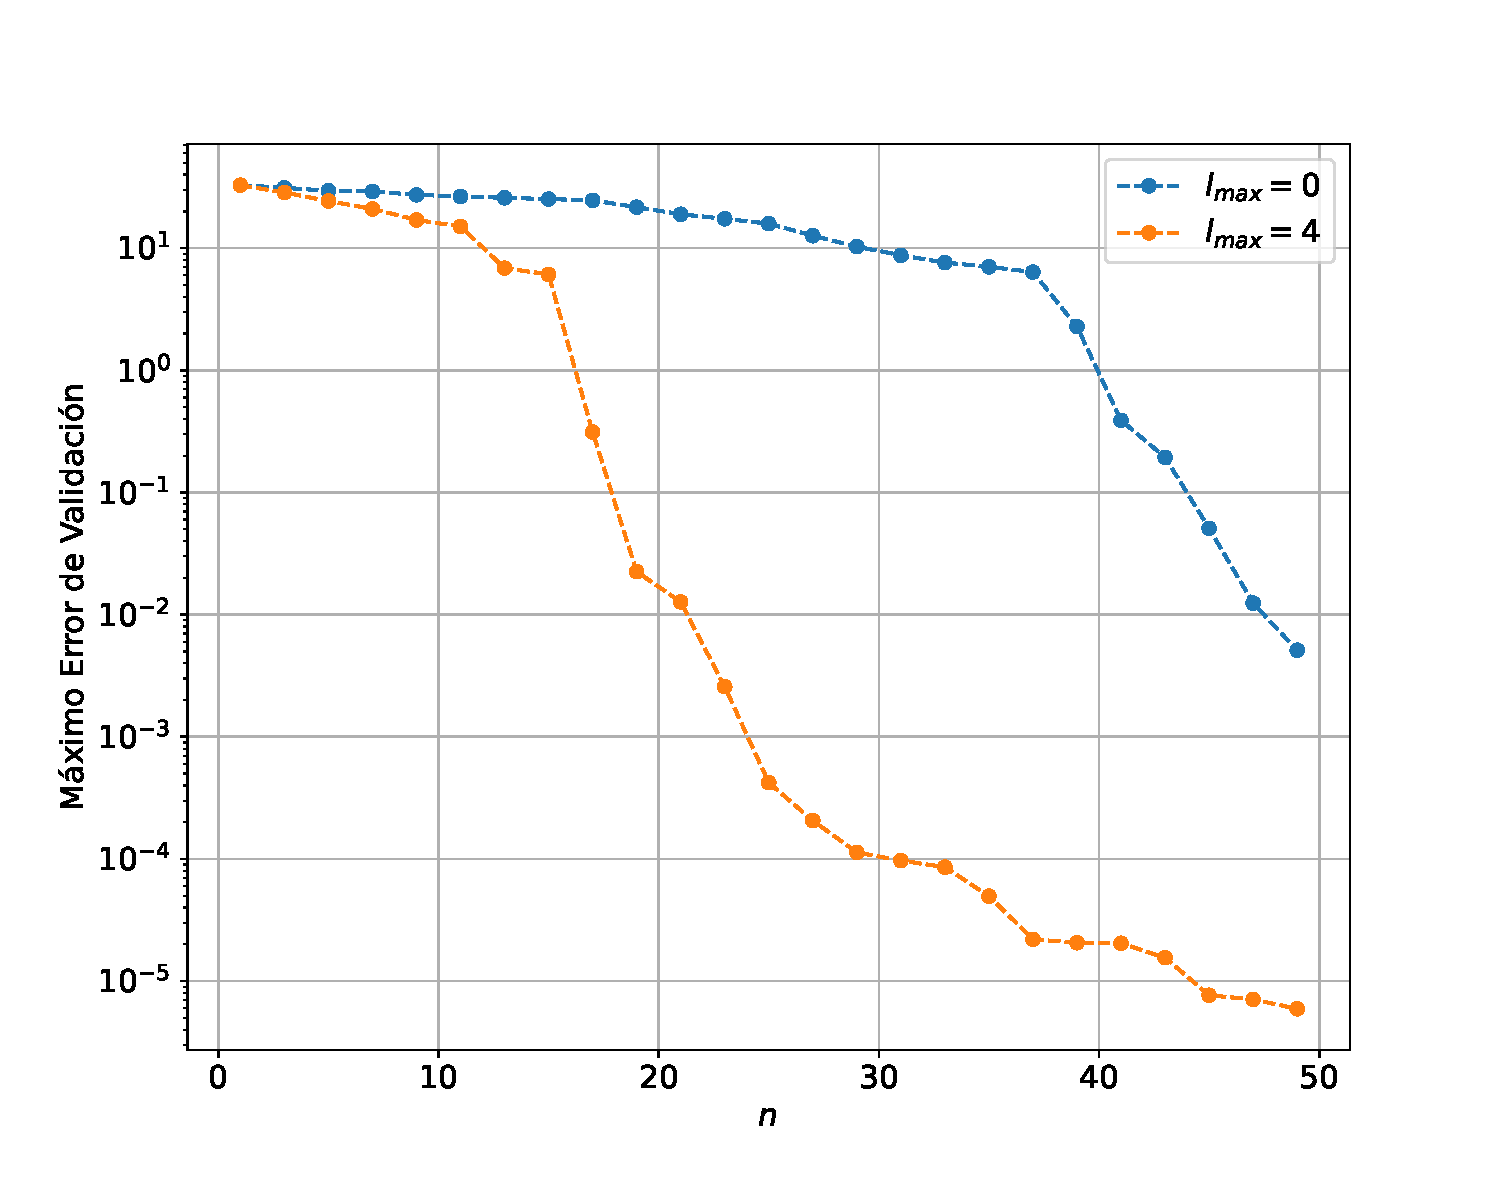
\includegraphics[width=.8\columnwidth, trim={0, 1.3cm, 0, 1.4cm}]{figs/l0vsl4.pdf}
\caption{Base global ($l_{max} = 0$) versus base con $l_{max} = 4$} para distintos valores de $n$.
\label{fig:l0vl4}
\end{figure}



\begin{figure}[h!]
\centering
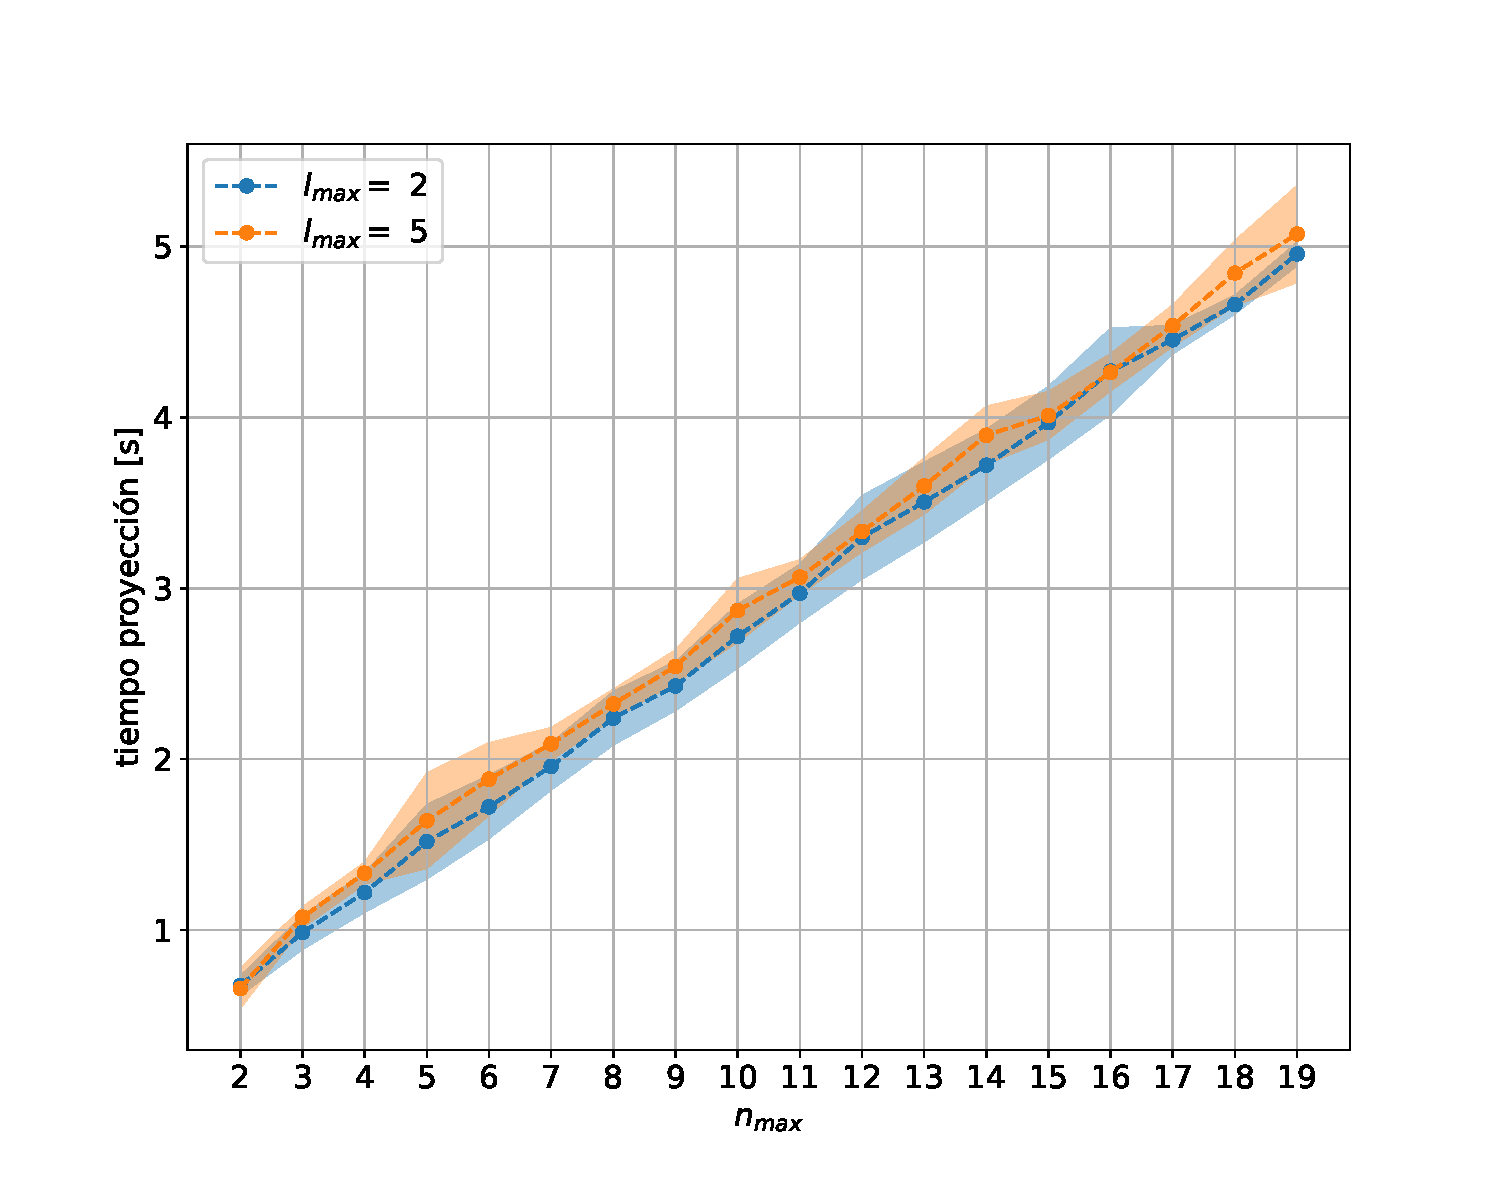
\includegraphics[width=.8\columnwidth ,trim={0, 1cm, 0, 1.2cm}]{figs/t_vs_nmax.pdf}
\caption{tiempos de proyección de un conjunto de validación a dos bases con distinto $l_{max}$ en función del $n_{max}$. En cada caso la linea de trazo representa el valor medio, y el área de color indica una desviación estandar desde el valor medio, para cada medición.}
\label{fig:t_vs_nmax}
\end{figure}


En la figura \ref{fig:t_vs_nmax} se graficó el tiempo de proyección de un conjunto de validación a dos bases \textit{hp-greedy} con distinto valor de $l_{max}$. Se observa que el tiempo es bastante lineal en relación al $n$ (elementos de las bases locales), y no parece ser afectado por $l_{max}$.



\begin{figure}[h!]
\centering
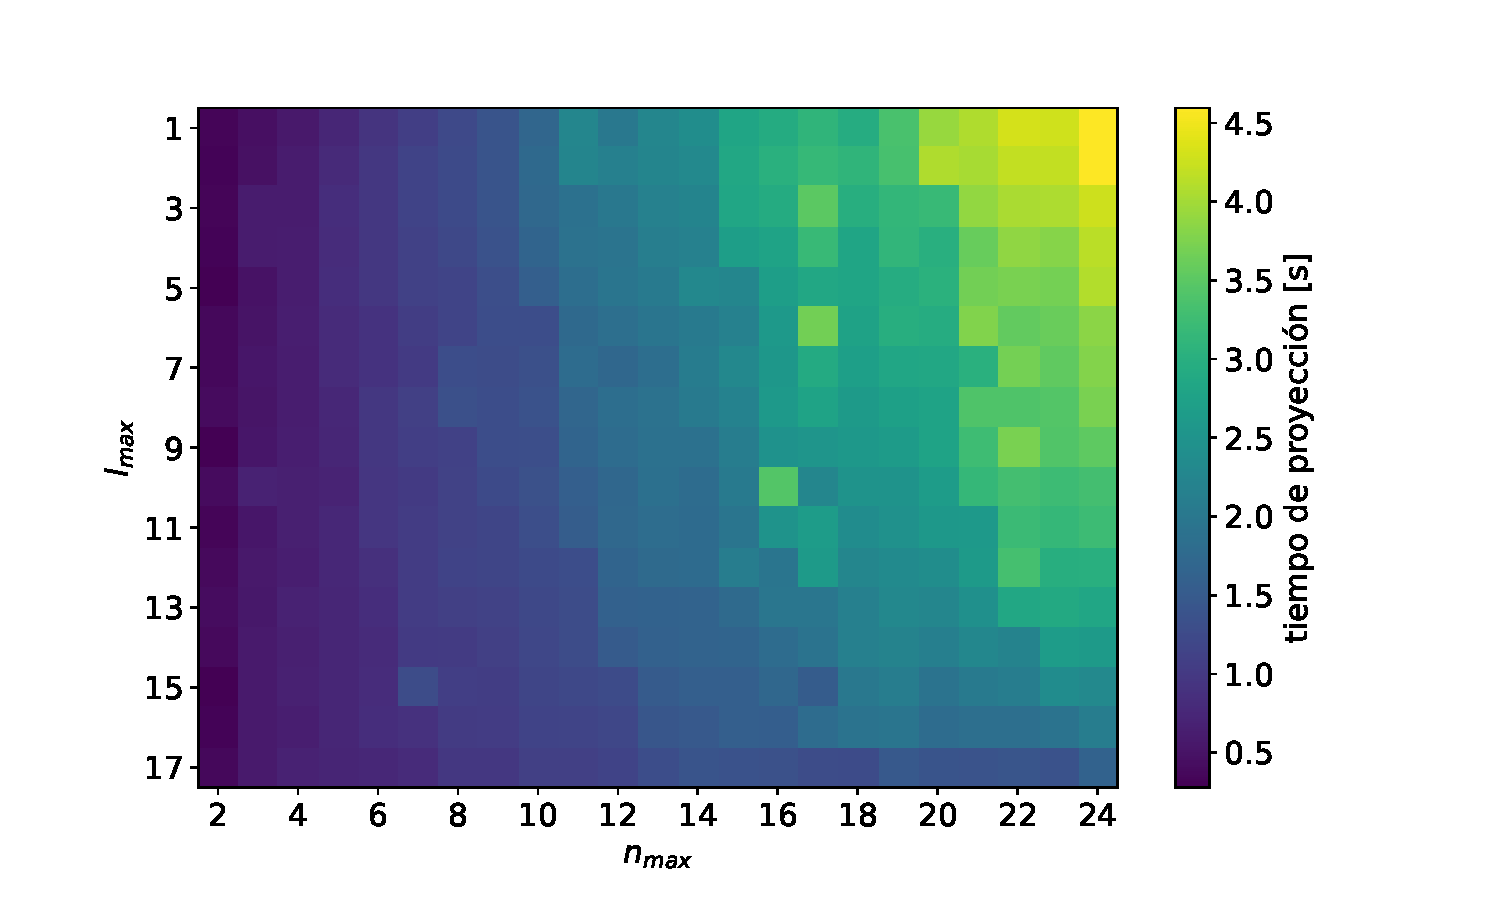
\includegraphics[width=.9\columnwidth, trim={0, 1cm, 0, 1.4cm}]{figs/nmax_lmax_t_grid.pdf}
\caption{Tiempo de proyección de un conjunto de validación para diferentes valores de $n_{max}$ y $l_{max}$}
\label{fig:t_grilla_nl}
\end{figure}



\subsection{Tiempo de Proyección para distintos valores de $n_{max}$ y $l_{max}$}

Para representar una función de onda a partir de una base \textit{hp-greedy} primero se debe buscar el subdominio (la hoja) correspondiente utilizando los puntos de anclaje y luego proyectar la función a la base local encontrada. 

En este proceso, el trabajo de cómputo relevante es la proyección a la base local (que es independiente de $l_{max}$), que involucra calcular $n$ coeficientes para una base local de $n$ elementos. Por lo tanto el tiempo de proyección será afectado por $n_{max}$ en mucha mayor medida que por $l_{max}$. 

En la figura \ref{fig:t_grilla_nl} se puede ver el tiempo de proyección para diferentes valores de $n_{max}$ y $l_{max}$. En los primeros valores de $l_{max}$, con $l_{max} \leq 5$, se observa un comportamiento similar al descrito anteriormente, donde el tiempo depende casi únicamente de $n_{max}$. Sin embargo al aumentar el $l_{max}$ se observa que el tiempo disminuye. 


Este comportamiento es consecuencia de la baja cantidad de elementos en el conjunto de entrenamiento en relación a la cantidad total de elementos en las bases hojas. 
Suponiendo un árbol denso (todas las bases tienen $n_{max}$ elementos y todas las hojas tienen profundidad $l_{max}$), habrá un total de $n_{max} \times 2^{l_{max}}$ elementos entre todas las hojas. 

Para obtener la Figura \ref{fig:t_grilla_nl} se utilizó un conjunto de entrenamiento con 1400 funciones de onda, por lo que al llegar a unos valores de $l_{max} = 6$ y $n_{max} = 24$ en total debería haber 1536 elementos entre todas las bases locales de las hojas. Es decir, más elementos de base que ondas en el conjunto de entrenamiento. Por lo tanto al aumentar el $l_{max}$ llegará un punto en el que no habrá suficientes elementos en el conjunto de entrenamiento para que cada base local tenga $n_{max}$ elementos. De forma que las bases locales serán cada vez más pequeñas, lo que dará lugar a un tiempo de proyección menor.



\subsection{Hiperparámetros}

\begin{figure}[h!]
\centering
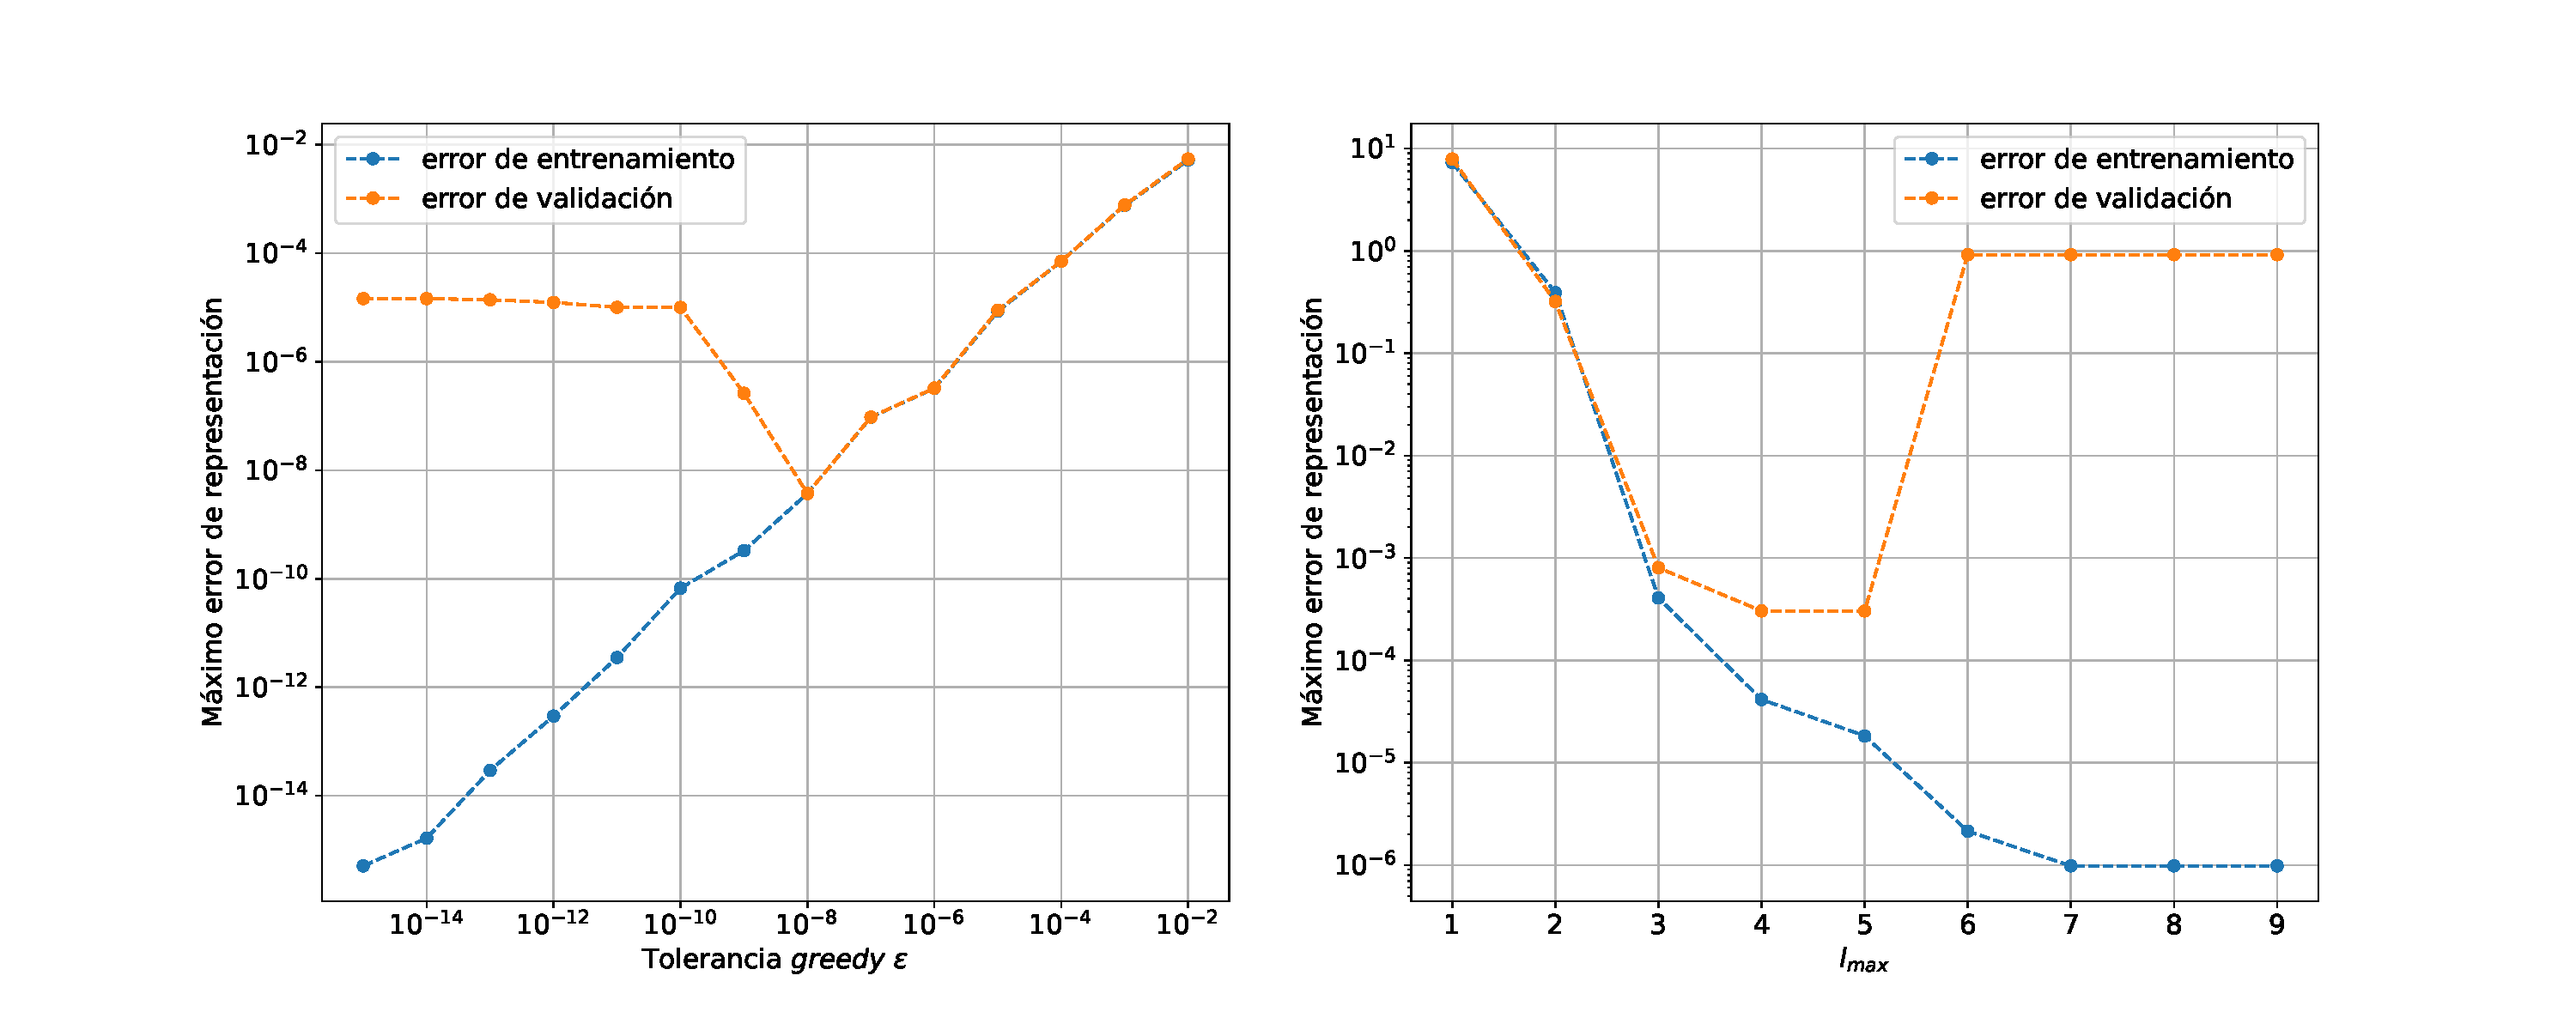
\includegraphics[width=1\columnwidth ,trim={2cm, 1cm, 1cm, 1.2cm}]{figs/overfit.pdf}
\caption{Ejemplos de \textit{sobreajuste}. A la izquierda variando $\varepsilon$ con $(n_{max}, l_{max}) = (25, 19)$ en un conjunto de parámetro unidimensional $(\lambda_i = q_i)$. A la derecha variando $l_{max}$ con $(n_{max}, \varepsilon) = (20, 1\times10^{-6})$ en un conjunto de parámetro bidimensional$(\lambda_{ij} = (q_i, \chi_{z_j})) $.}
\label{fig:overfit}
\end{figure}

Al momento de construir una base \textit{hp-greedy} entran en juego cuatro hiperparámetros. Los primeros tres son los parámetros de parada;
\begin{itemize}
\item $\bm{n_{max}}:$ determina la cantidad máxima de elementos para cada base local. A mayor cantidad de elementos el error de representación será menor, pero el tiempo requerido para proyectar un conjunto de validación a la base depende casi exclusivamente de este hiperparámetro.
\item $\bm{l_{max}}:$ determina la máxima profundidad de las hojas del árbol. En general al aumentar $l_{max}$ disminuye el error de representación, pero valores muy elevados junto a cierta combinación de hiperparámetros pueden dar lugar a sobreajustes en el modelo, un ejemplo de esto se puede ver en la figura \ref{fig:overfit}. Este es un comportamiento típico de las estructuras arbóreas.
\item $\bm{\varepsilon}$: la tolerancia \textit{greedy} interviene tanto en el tamaño de las bases locales como en la profundidad de las hojas del árbol. Un valor de $\varepsilon$ demasiado bajo también puede dar lugar a sobreajuste, sobre todo con valores muy altos de $l_{max}$. Un valor de $\varepsilon = 0$ implica que se obtiene un árbol totalmente denso, determinado únicamente por $n_{max}$ y $l_{max}$, y al aumentar el valor de $\varepsilon$ se puede pensar en la analogía de podar un árbol, de forma que se previene el sobreajuste.
\end{itemize}

Al cuarto hiperparámetro se le da el nombre de \textit{\textbf{semilla}} y en este trabajo se la denota con $\bm{\hat{\Lambda}_0}$ para diferenciarla de la semilla de una base local, denotada por $\Lambda_1$;

\begin{figure}[h!]
\centering
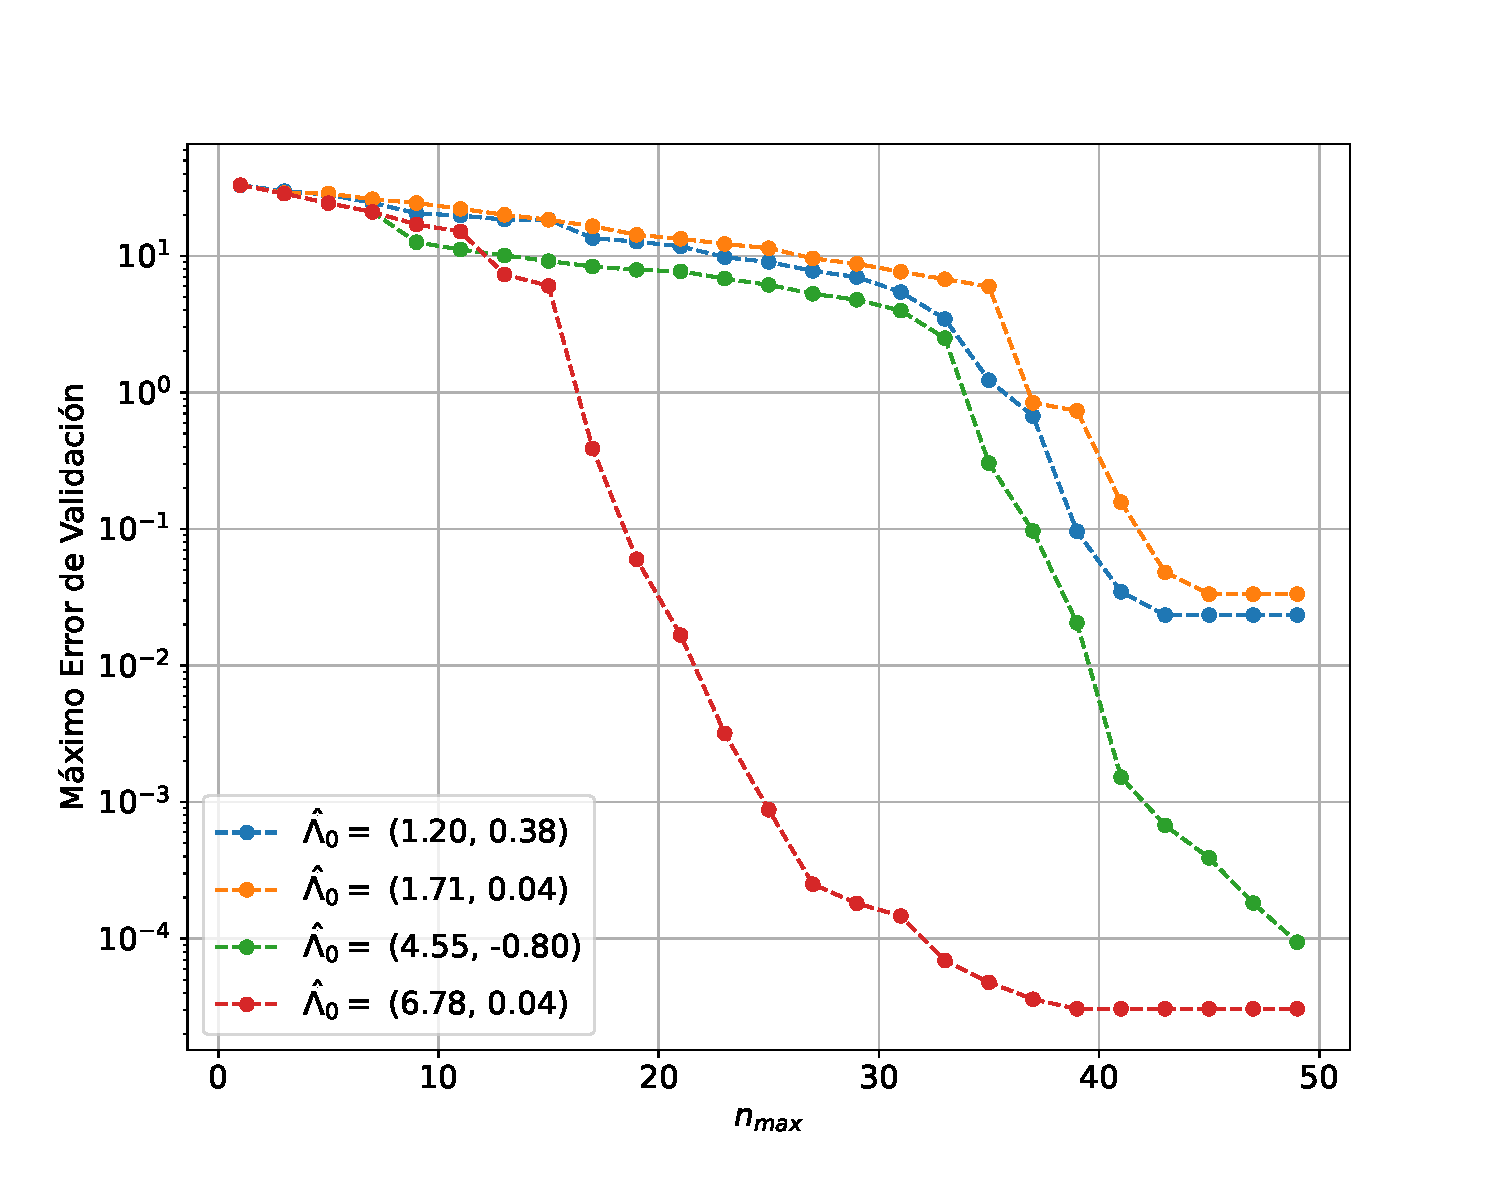
\includegraphics[width=.8\columnwidth ,trim={1.1cm, 1.1cm, 1.2cm, 1.2cm}]{figs/Semillas_v_nmax_2D.pdf}
\caption{Error de validación para diferentes semillas $\hat{\Lambda}_0 = (q_0, \chi_{z_0})$.}
\label{fig:seeds0}
\end{figure}

\begin{itemize}
\item $\bm{\hat{\Lambda}_0}$: la semilla no es más que el primer parámetro \textit{greedy} de la base global. En cada base local, el primer parámetro \textit{greedy} no es relevante, pero en el caso de las bases \textit{hp-greedy} cada semilla dará lugar a una división diferente del dominio de parámetros. En la figura \ref{fig:seeds0} se puede ver como cuatro semillas diferentes dan lugar a cuatro curvas de error con distinta convergencia. En la figura \ref{fig:seeds_part}, por otro lado, se observa el resultado de la partición del dominio para tres semillas diferentes. En general las semillas que mejor funcionan (con el conjunto de datos utilizado) son las que logran una partición regular del dominio de parámetros. 
\end{itemize}

En caso de trabajar con un espacio de parámetros bidimensional la semilla será $\hat{\Lambda}_0 = (q_0, \chi_{z_0})$,  con $q$ la relación entre masas y $\chi_z$ el espín en la dirección $z$. 

\begin{figure}[h!]
\centering
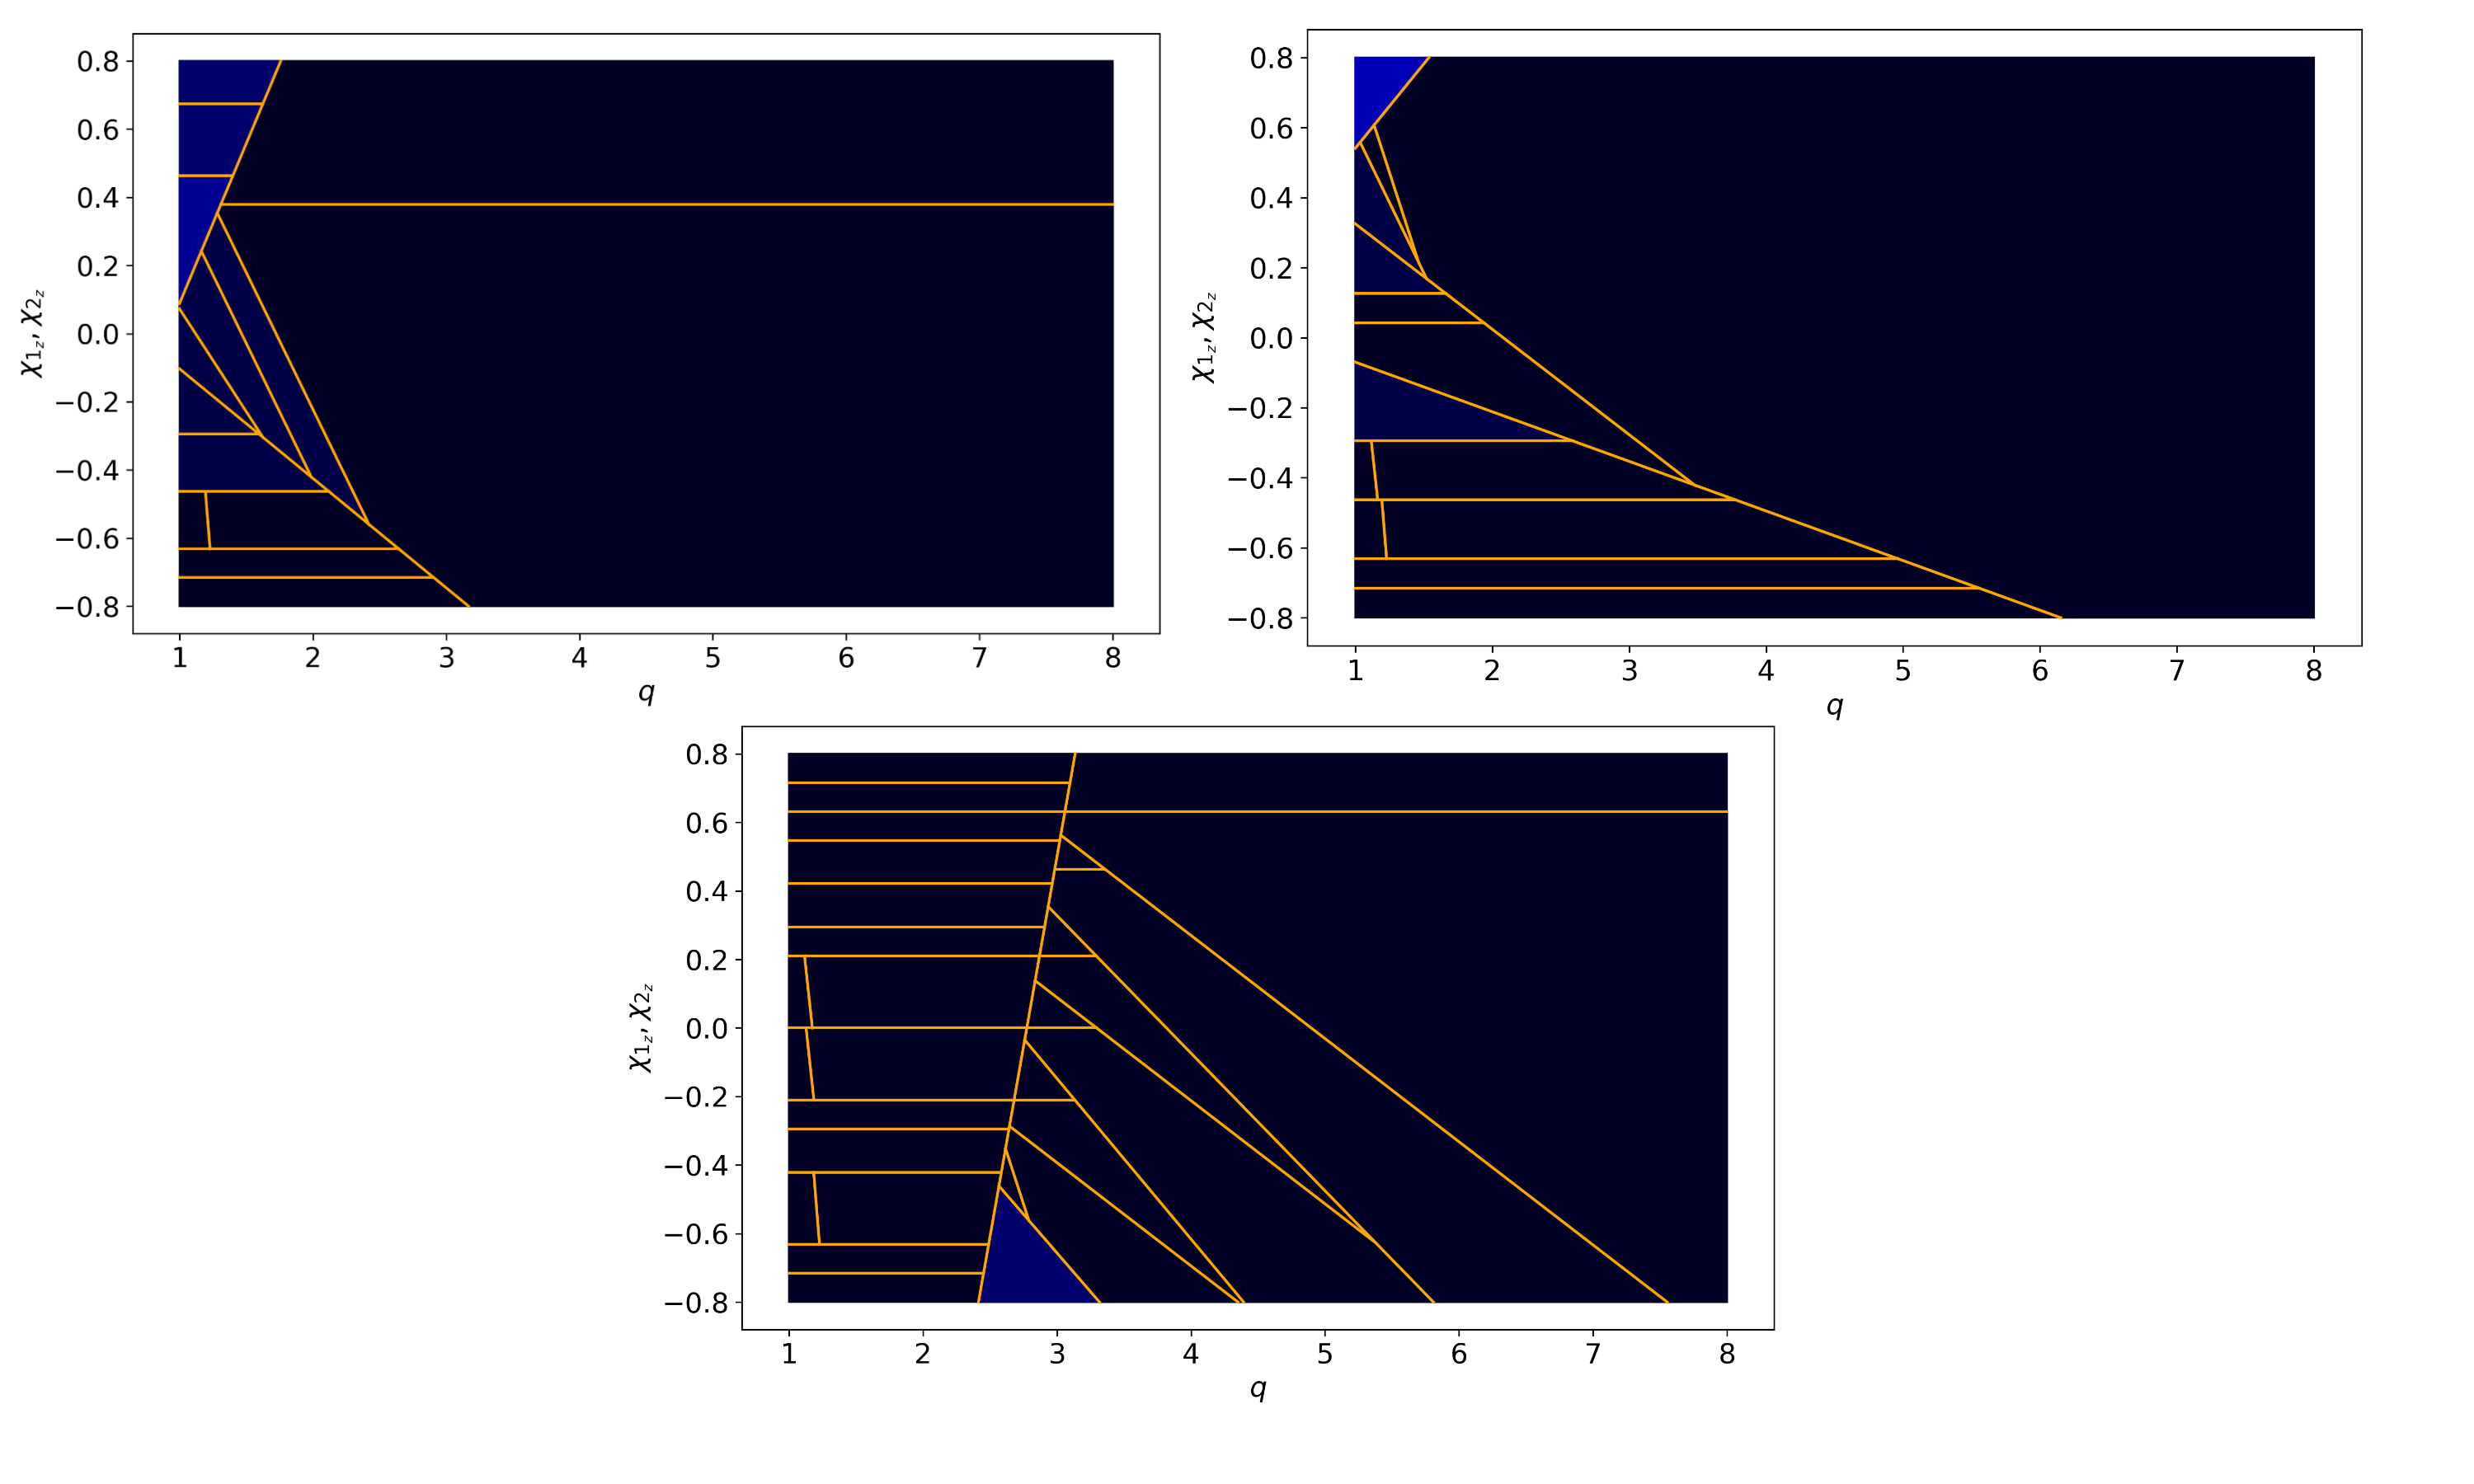
\includegraphics[width=1.05\columnwidth ,trim={1.1cm, 1cm, 1cm, 1.2cm}]{figs/3_semillas_particion.png}
\caption{Partición del espacio de parámetros para tres semillas diferentes; a la izquierda $\hat{\Lambda}_0 = ($1.2$,\  $0.38$)$, a la derecha $\hat{\Lambda}_0 = ($1.71$,\  $0.04$)$ y al centro $\hat{\Lambda}_0 =($4.55$,  -$0.8$)$. Recordar que $\hat{\Lambda}_0 = (q_0, \chi_{z_0})$.}
% Recordar que $\hat{\Lambda}_0 = (q_0, \Chi_0)$.
\label{fig:seeds_part}
\end{figure}
% Capitulo 3
\section{Optimización de Hiperparámetros}

Sea $f: X \rightarrow \mathbb{R}$ una función que devuelve el máximo error de validación de un modelo entrenado a partir de una combinación de hiperparámetros $\textbf{x} \in X$, se desea encontrar $\hat{\textbf{x}}$:

\[
\hat{\textbf{x}} = arg \min_{\textbf{x} \in X} f(\textbf{x})
\]

Es decir, se busca encontrar la combinación óptima de hiperparámetros dentro de un dominio $X$ para obtener el mínimo error de representación en un dado conjunto de validación.En el caso de la construcción de una base \textit{hp-greedy} óptima: 

\[
\textbf{x} = (n_{max}, l_{max}, \varepsilon, \hat{\Lambda}_0)
\]

El hiperparámetro de mayor interés es sin duda la $semilla$, pues a primera vista no hay una forma obvia de elegir su valor óptimo. Además una semilla óptima para una combinación de $(n_{max_1}, l_{max_1})$ no lo será necesariamente para otra combinación $(n_{max_2}, l_{max_2})$.

También se observó que en ciertas situaciones un valor muy elevado de $l_{max}$ o muy pequeño de la $tolerancia$ $greedy$ pueden conducir a un modelo \textit{sobreajustado}. Por esto es de interés realizar una optimización que involucre a la totalidad de los hiperparámetros dentro del dominio $X$. 


El problema al momento de realizar esta optimización es que la función $f$ no es una función analítica, sino es que es el resultado de entrenar el modelo y evaluar el error de representación con un conjunto de validación, lo que la hace costosa de evaluar (computacionalmente hablando). Esta sección se centrará en la \textbf{optimización Bayesiana} \cite{7352306, https://doi.org/10.48550/arxiv.1012.2599}, un método que intenta reducir al mínimo el número de evaluaciones de $f$ para encontrar $\hat{\textbf{x}}$ y se puede colocar dentro de una categoría llamada optimización secuencial basada en modelos, o \textbf{SMBO}\cite{dewancker2015bayesian,NIPS2011_86e8f7ab} (\textit{Secuential Model-Based Optimization}).


Además existen dos métodos muy utilizados que no utilizan modelos, los cuales son la busqueda exaustiva (o \textit{grid search}) y la búsqueda aleatoria. Antes de hablar de la optimización Bayesiana se introducirá brevemente dl método de la búsqueda exhaustiva para luego realizar una comparación entre ambos métodos en un problema de optimización relativamente sencillo.


\subsection{Búsqueda Exhaustiva}

 
 
 
 La búsqueda exhaustiva o \textit{grid search} consiste en probar todas las combinaciones posibles dentro de un espacio de hiperparámetros para seleccionar la solución óptima. Es decir que si se quiere buscar la combinación óptima de $(n_{max}, l_{max})$ para un rango de valores $n_{max} \in N,$ $l_{max} \in L$ se deberán probar todas las combinaciones posibles del producto cartesiano $N \times L = \{(n_{max}, l_{max}) | n_{max} \in N, l_{max} \in L\}$. 
 
La ventaja de este método está en que el resultado óptimo está garantizado, pues se pueden comparar todos los resultados entre sí y elegir el mejor. El problema es que, como se mencionó, la función $f$ es costosa de evaluar, y por otro lado el número de combinaciones posibles escala exponencialmente con cada hiperparámetro extra a optimizar (además se debe tener en cuenta que la semilla $\hat{\Lambda}_0$ tendrá generalmente más de una dimension).

Por estas razones la búsqueda exhaustiva no será un método viable en la mayoría de los casos que son de interés para este trabajo. Sin embargo se puede poner a prueba con casos simplificados para luego comparar los resultados con otros métodos más eficaces.

\begin{figure}[h!]
\centering
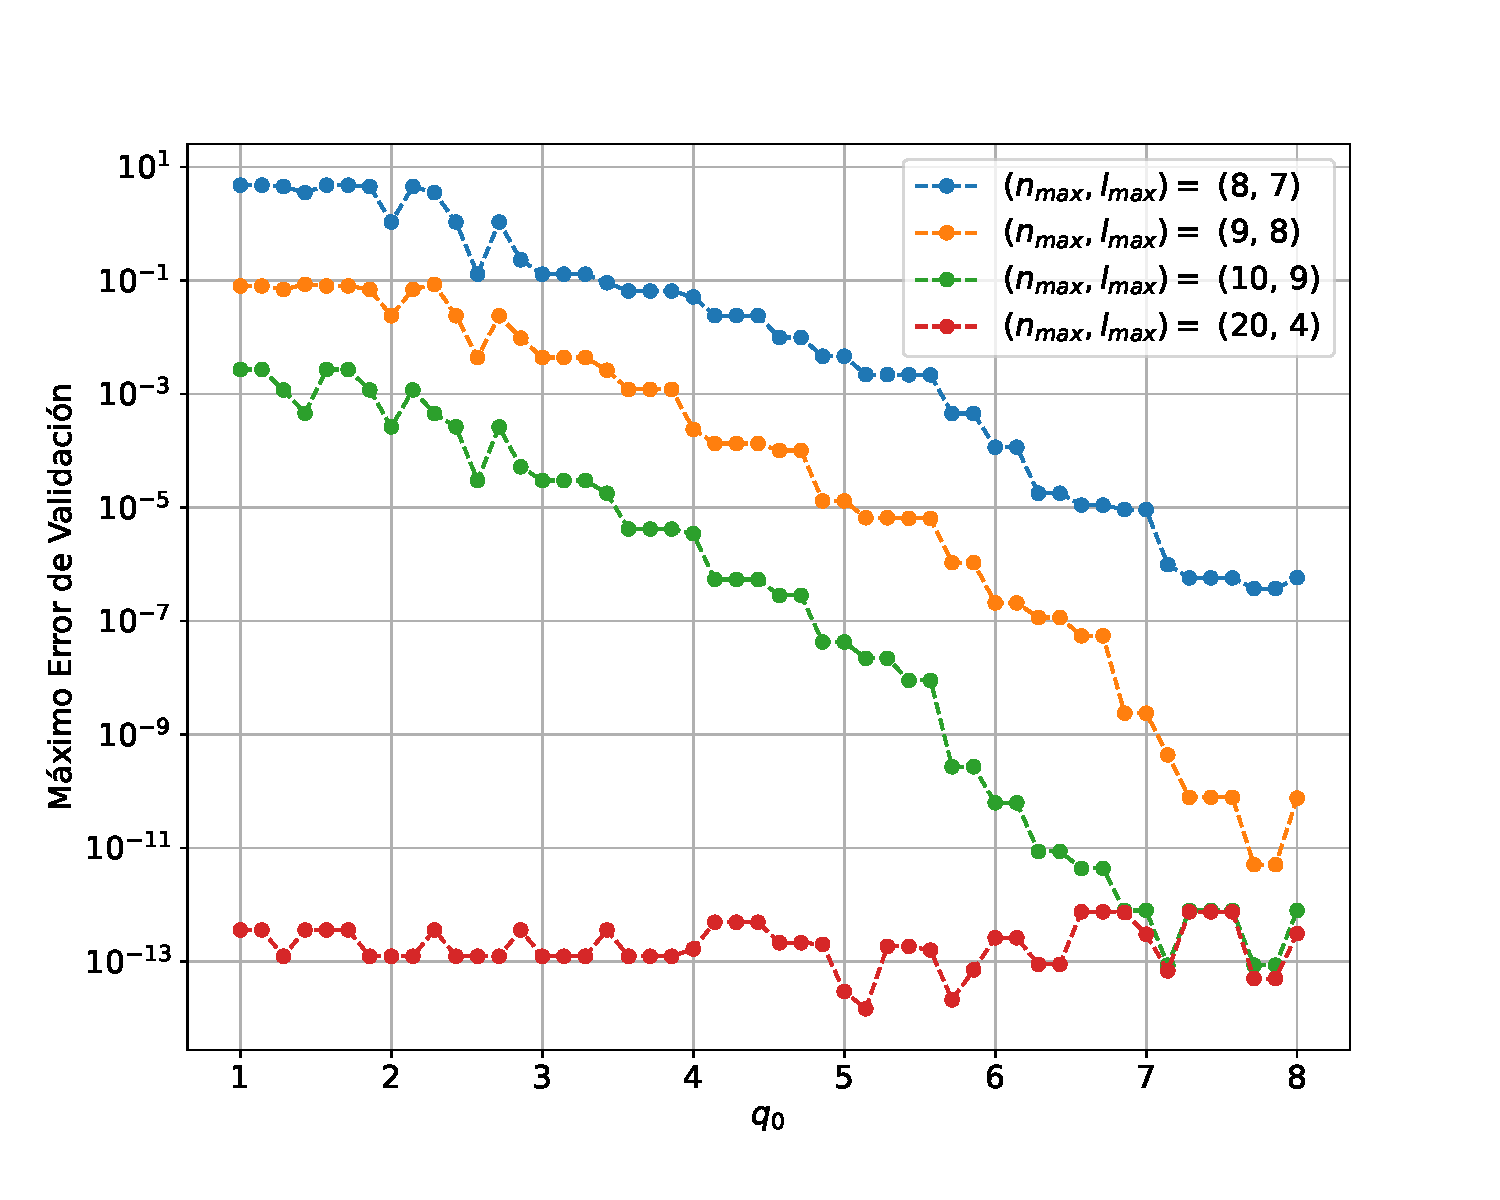
\includegraphics[width=.8\columnwidth, trim={1.1cm, 1cm, 1cm, 1.2cm}]{grid_seeds_0.pdf}
\caption{Variación de la semilla $q_0$ para distintas combinaciones de $(n_{max}, l_{max})$}
\label{fig:grid_seed_0}
\end{figure}

Por ejemplo, para un conjunto de entrenamiento con cincuenta ondas equidistantes en el espacio del parámetro unidimensional $q: 1 < q < 8$, se quiere optimizar el error de representación para un conjunto de validación con mil ondas. Los hiperparámetros a optimizar son $\textbf{x} = (n_{max}, l_{max}, \hat{\Lambda}_0)$, dejando $\varepsilon$ fijo en $1\times 10^{-12}$ para simplificar la búsqueda, que se realiza en los siguientes intervalos:

\begin{align*}
n_{max} &\in [5, 20],\\
l_{max} &\in [1, 10],\\
\hat{\Lambda}_0 &\in \{q_0 \ | \ q_0 = 1 + i \Delta q, \ i\in \mathbb{N} : 0 \le i \le 49, \ \Delta q = 7/49 \}.
\end{align*}

Son 16 valores de $n_{max}$, 10 valores de $l_{max}$ y 50 para $q_0$ ($\hat{\Lambda}_0 = q_0$). Lo que hace un total de 8000 combinaciones posibles.



\begin{figure}[h!]
\centering
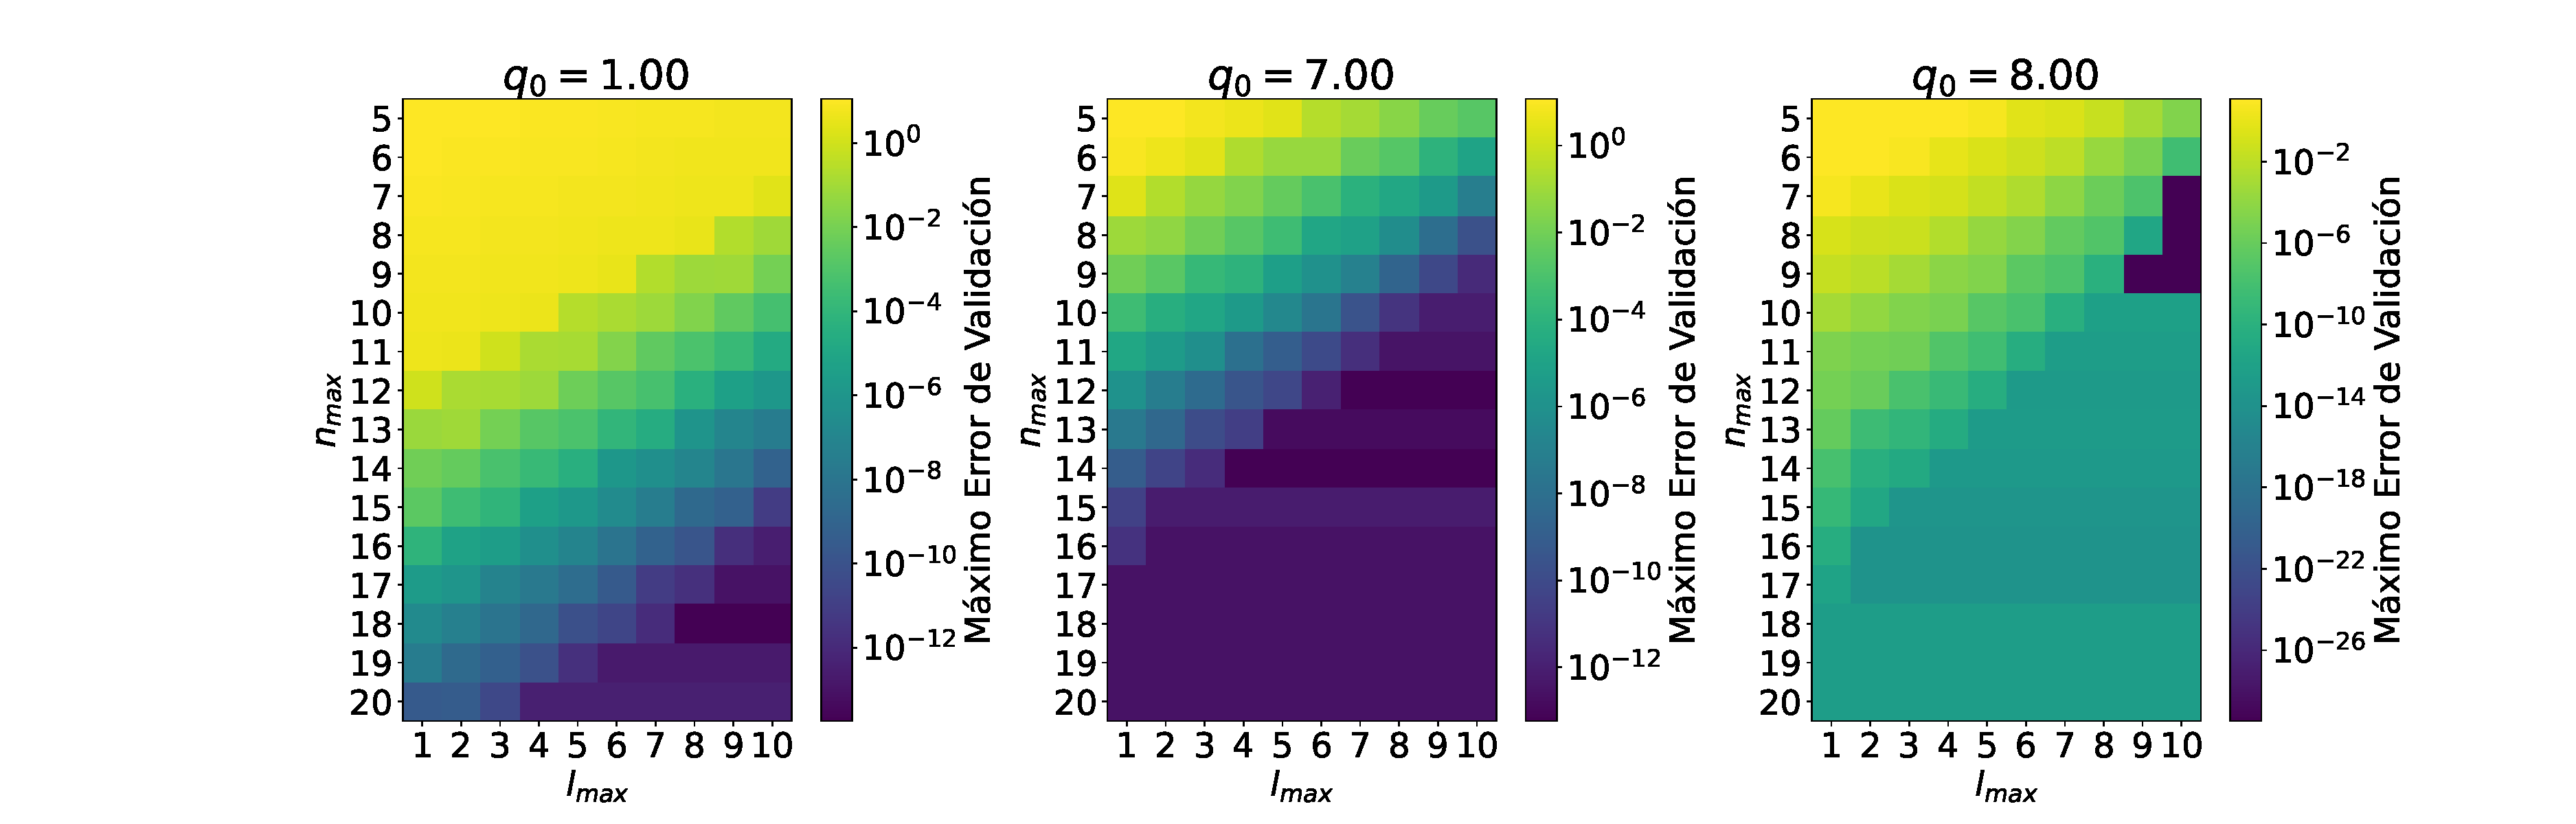
\includegraphics[width=1.05\columnwidth, trim={8cm, 1cm, 5cm, 1.1cm}]{grid_3_seeds.pdf}
\caption{Máximo error de validación en función de $n_{max}$ y $l_{max}$ para tres diferentes semillas $q_0$. }
\label{fig:grid_3_seeds}
\end{figure}

Si bien no se puede graficar el error en función de los tres hiperparámetros a la vez, se puede obtener bastante información al dejar fijo uno o dos hiperparámetros. Por ejemplo en la figura \ref{fig:grid_seed_0} se ven los resultados de variar únicamente la semilla para diferentes combinaciones de $n_{max}$ y $l_{max}$. Se observa que en este conjunto de datos la semilla suele ser óptima a valores cercanos a $q_0 = 8$, pero a la vez al aumentar el $n_{max}$ la influencia de la semilla es menor; con $(n_{max}, l_{max})=(20, 4)$ hay una diferencia de un orden de magnitud entre la mejor y la peor semilla, mientras que con $(n_{max}, l_{max})=(10, 9)$, por ejemplo, hay una diferencia de diez ordenes de magnitud.

Luego, en la figura \ref{fig:grid_3_seeds} se observa el error de validación en función de las combinaciones posibles de  $n_{max}$ y $l_{max}$ para tres diferentes semillas. A la derecha, con $q_0=8$ se observa el mejor error de representación obtenido en la búsqueda exhaustiva, con un valor de $4\times10^{-30}$ (el cual se obtuvo para 16 combinaciones de hiperparámetros), casi 15 ordenes de magnitud menor que el siguiente mejor error.


\subsection{Optimización Bayesiana}

\begin{figure}[h!]
\centering
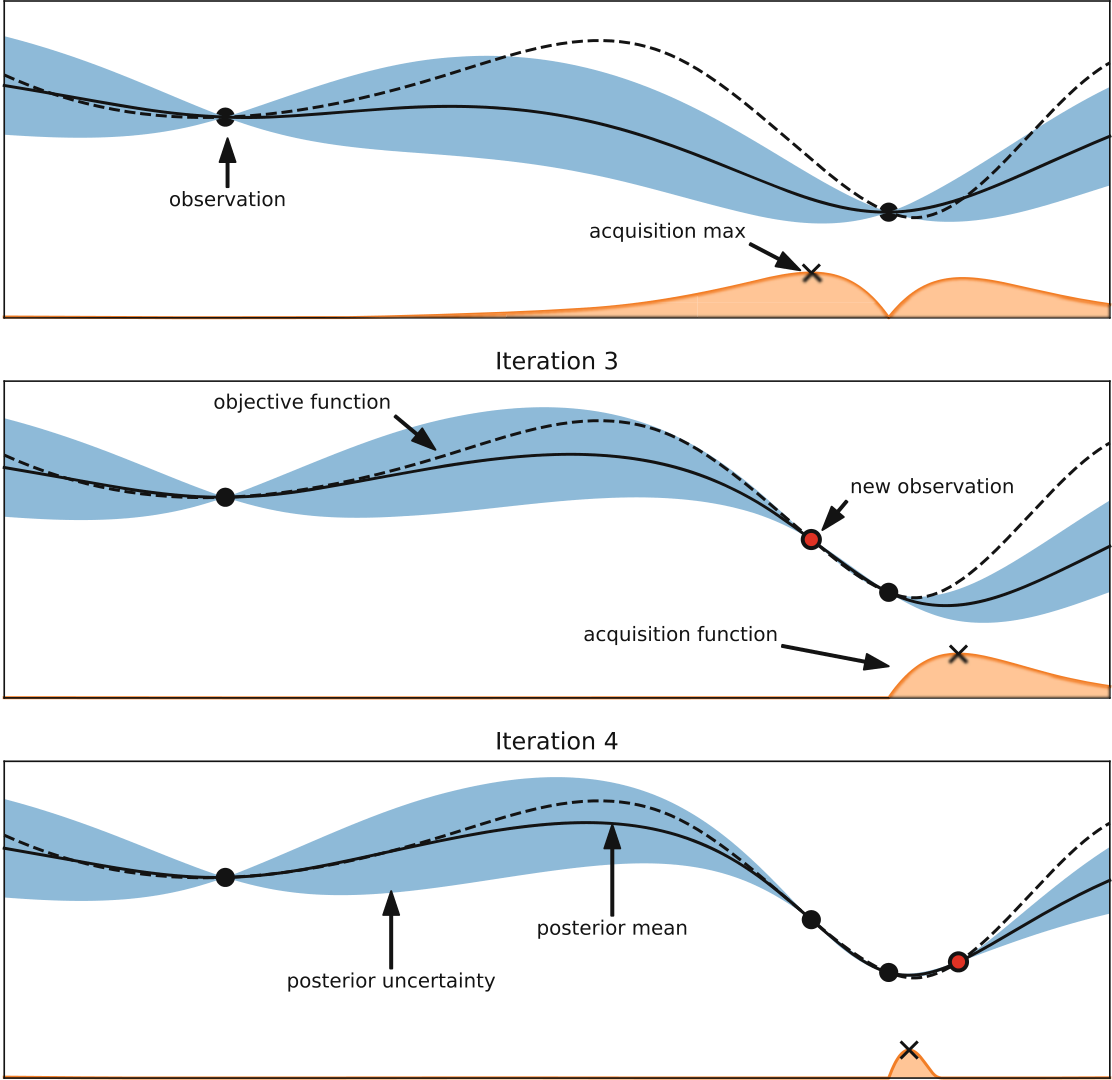
\includegraphics[width=.7\columnwidth]{bayesian.png}
\caption{En la figura se observan tres iteraciones de una optimización bayesiana para una función sencilla con parámetro unidimensional. En linea punteada está representada la función real, mientras que con linea gruesa se representa el valor medio del modelo estadístico (en este caso construido utilizando procesos gaussianos). El área pintada en azul representa la incertidumbre del modelo, que tiende a cero en los puntos que representan las observaciones realizadas. Debajo se puede ver una función de adquisición en color naranja, que indica el siguiente punto a evaluar \cite{Feurer2019}.}
\label{fig:bayesian}
\end{figure}

La optimización bayesiana es un método que utiliza la información de todas las evaluaciones realizadas de la función $f$ para decidir que valor de $\textbf{x}$ evaluar a continuación, reduciendo así el número necesario de evaluaciones de $f$ para encontrar el mínimo.

Para explicar como funciona este método se parte de un formalismo llamado \textbf{optimización secuencial basada en modelos}, que no es más que una generalización de la optimización bayesiana.


En la optimización secuencial basada en modelos cada evaluación de la función $f$ se decide en base al conjunto $D$ de observaciones realizadas previamente. Esto se logra entrenando un modelo sustituto $\mathcal{M}$ en base al conjunto $D$, y luego utilizando una función $S$ llamada función de \textit{adquisición}, que decidirá el mejor punto a evaluar en la función real.

Se parte de un conjunto $D$ generado a partir de un muestreo de observaciones de la función $f$ de la forma $(\textbf{x}_j, f(\textbf{x}_j))$, a partir del cual se ajusta el modelo sustituto $\mathcal{M}$. Luego, maximizando la función de adquisición $S$ se elije el siguiente conjunto de hiperparámetros $\textbf{x}_i$ para evaluar la función $f$ y se agrega el par $(\textbf{x}_i, f(\textbf{x}_i))$ al conjunto de observaciones $D$. Una vez hecho esto se vuelve a ajustar el modelo $\mathcal{M}$ y se repite el proceso, que está explicado en forma de pseudocódigo en el algoritmo \ref{alg:SMBO}.


\begin{algorithm}
\caption{\texttt{SMBO}}
\label{alg:SMBO}
\begin{algorithmic}[1]
\Require $f, X, S,\mathcal{M}$
\State $D =$ InicializarMuestras$(f, X)$
\vspace{1mm}
\For{$i = 1, 2, ...$}
	\State $\mathcal{M} =$ AjustarModelo$(D)$
	\State $\textbf{x}_{i} = arg \max_{\textbf{x}\in X} \mathcal{S}(\textbf{x}, \mathcal{M})$ .
	\State $y_i = f(\textbf{x}_i)$	\Comment{Paso costoso}
	\State $D = D \cup \{(\textbf{x}_i, y_i)\}$
\EndFor
\vspace{3mm}

\end{algorithmic}
\end{algorithm}


Lo que caracteriza a la optimización bayesiana dentro del formalismo de la optimización secuencial basada en modelos, es justamente la creación del modelo.
En la optimización bayesiana se construye un modelo estadístico, donde se representa con  $P(y|\textbf{x})$ la predicción del modelo, siendo $y$ el resultado de una evaluación $f(\textbf{x})$. El nombre del método se debe a que para la construcción del modelo se utiliza el teorema de Bayes:
  
 \[
 P(y|\textbf{x}) = \frac{P(\textbf{x}|y) \ P(y)}{P(\textbf{x})}
 \]
 
 En la terminología bayesiana, se conoce a $P(y|\textbf{x})$ como probabilidad a posteriorí o \textit{posterior}, que es proporcional a la probabilidad a priori o \textit{prior} $P(y)$ por la función de verosimilitud o \textit{likelihood} $P(\textbf{x}|y)$. La probabilidad $P(\textbf{x})$ es una probabilidad marginal que sirve como factor de normalización, por lo que no es realmente relevante a la hora de encontrar valores extremos.


\subsubsection*{Procesos Gaussianos}

\begin{figure}[h!]
\centering
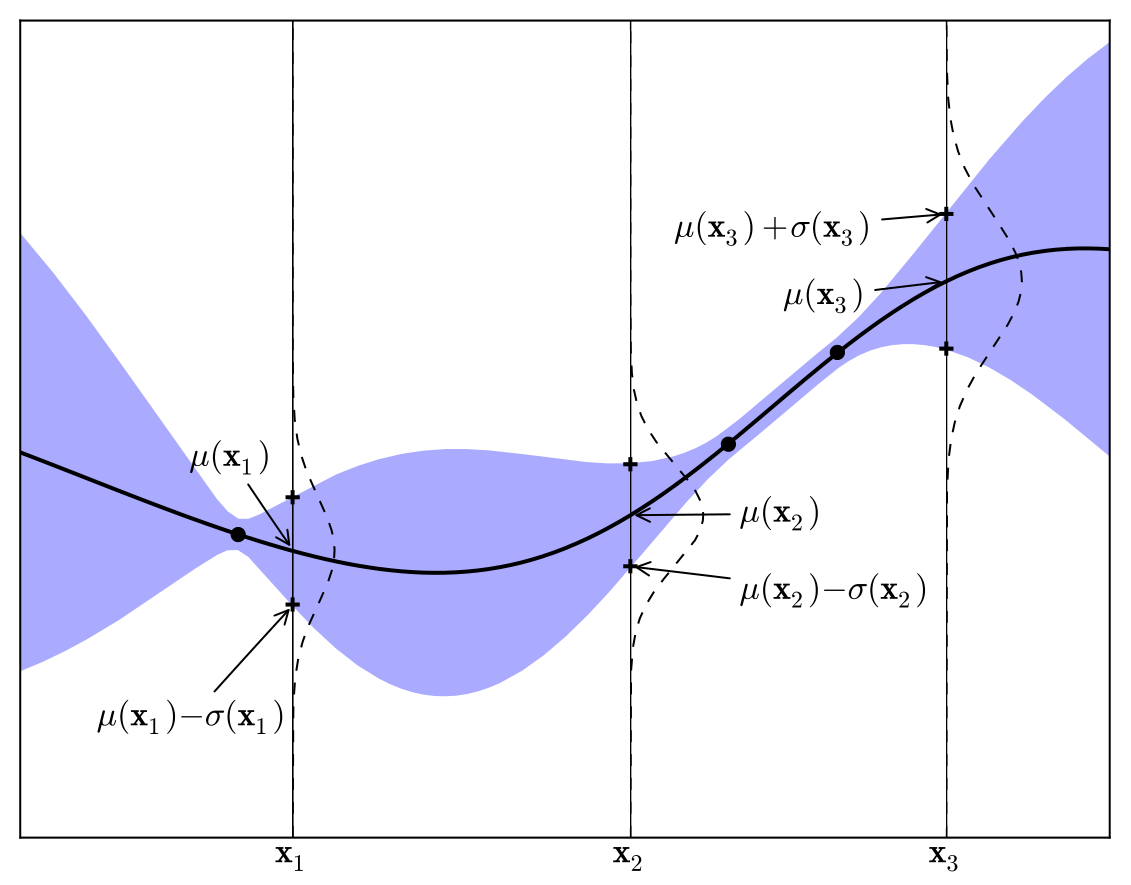
\includegraphics[width=.8\columnwidth]{gaussian.png}
\caption{Proceso Gaussiano unidimensional con tres observaciones representadas por los puntos negros. La linea gruesa representa la media del modelo predictivo y la zona azul la varianza en cada caso. Se representa con linea de trazo las distribuciones normales para los valores $x_1, x_2,$ y $x_3$\cite{https://doi.org/10.48550/arxiv.1012.2599}.}
\label{fig:gaussian}
\end{figure}

Una opción muy utilizada para la construcción del \textit{prior} y actualización del \textit{posterior} son los procesos gaussianos. Una forma sencilla de entender un proceso gaussiano es pensarlo como una función que para cada valor de $x$ devuelve la media $\mu(x)$ y la varianza $\sigma(x)$ de una distribución normal, en el caso particular de que $x$ sea unidimensional (ver figura \ref{fig:gaussian}). Con $\textbf{x}$ multidimensional, se obtiene una distribución normal multivariable, caracterizada por el vector $\bm{\mu}(\textbf{x})$ y la matriz de covarianza $\Sigma(\textbf{x}, \textbf{x}')$.

Sin embargo en este trabajo no se utilizan procesos gaussianos, principalmente porque parten del supuesto de que $f$ es continua. Para una introducción a la optimización bayesiana con procesos gaussianos ver \cite{https://doi.org/10.48550/arxiv.1012.2599}.

\subsubsection*{Estimador de Parzen con Estructura Arbórea} 
 
 
 El estimador de Parzen con estructura arbórea o \textbf{TPE} (\textit{Tree-Structured Parzen Estimator}) \cite{NIPS2011_86e8f7ab} es una estrategia que modela el \textit{prior} $P(y)$ a partir de densidades no paramétricas según el espacio de búsqueda, que en este caso son intervalos discretos. 
 
Por otro lado se modela $P(\textbf{x}|y)$ con dos distribuciones creadas a partir de las observaciones $D$ (de aquí el nombre de estructura arbórea):

\begin{equation}
P(\textbf{x}|y) =
	\begin{cases}
		\ell (x) & \text{si } y <y^{*} \\
		g(x) & \text{si } y \geq y^{*},
	\end{cases}
\end{equation}

con $y^{*}$ un valor por encima del mejor valor observado de $f(\textbf{x}9$, que se elije a partir de una fracción $\gamma$ de los valores observados $y$ tal que $P(y<y^{*}) = \gamma$.
 
\subsubsection*{Mejora Esperada: Función De Adquisición} 
 
%Debido a que la función $f$ no será necesariamente convexa, y seguramente tendrá varios mínimos locales, es necesario mantener un equilibrio entre la explotación y la exploración, es decir, explorar los mínimos tentativos sin dejar de lado las zonas inexploradas, en donde podría haber algún mínimo por descubrir. De esto se encarga la función de adquisición.
Para la elección de los puntos a evaluar en la función real se maximiza la función de adquisición $S$. Existen varias propuestas de funciones de adquisición, pero en este caso se utiliza la \textbf{mejora esperada} o EI(\textit{Expected Improvement}) \cite{EI1}. Sea $y^*$ un valor de referencia, se define a la mejora con respecto a $y^*$ como

\begin{equation}
I_{y^*}(\textbf{x}) = \max(y^*-y,0),
\end{equation}

Por lo tanto, la mejora esperada se obtiene calculando la media de $I_{y^*}(\textbf{x})$

\begin{equation}
EI_{y^*}(\textbf{x}) = E[\max(y^*-y,0)]= \int_{-\infty}^{\infty} \max(y^*-y,0) p(y|\textbf{x}) \ dy
\end{equation}
 
[Seguir con el resultado de EI aplicado al TPE]
 


 




\begin{figure}[h!]
\centering
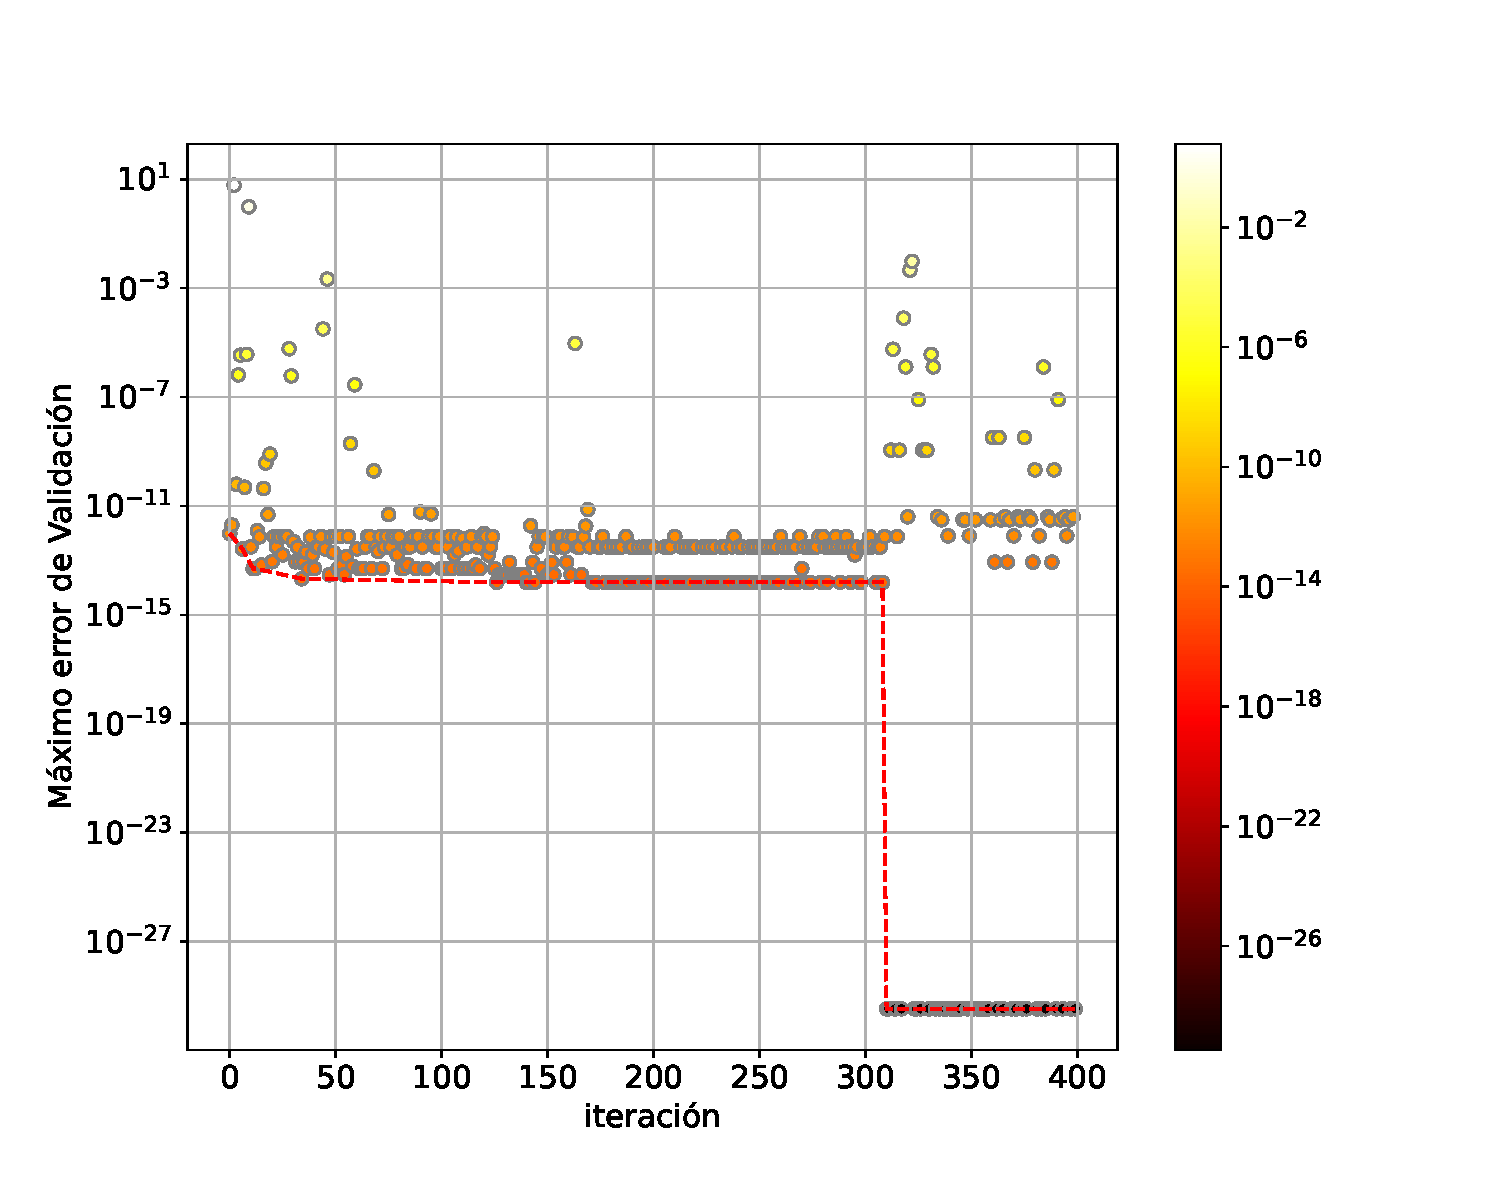
\includegraphics[width=.9\columnwidth, trim={1cm, 1cm, 1cm, 1.1cm}]{opt_1d_value.pdf}
\caption{caption }
\label{fig:optuna_1_value}
\end{figure}

  

\begin{figure}[h!]
\centering
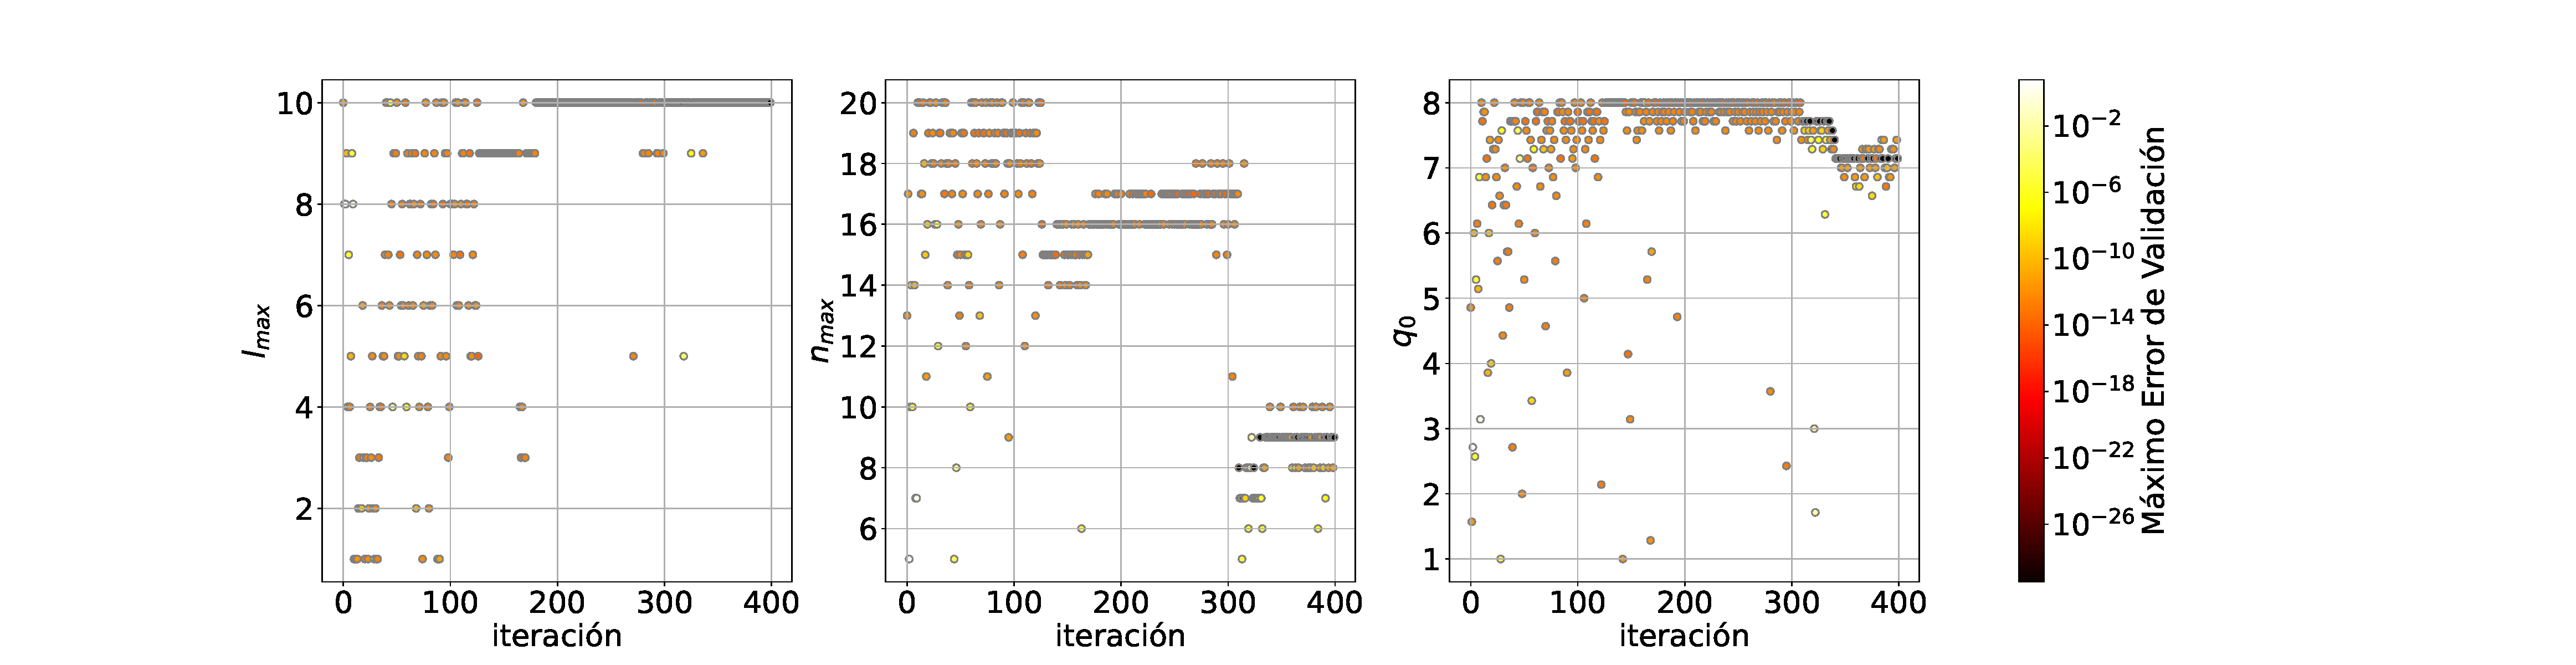
\includegraphics[width=1.05\columnwidth, trim={10cm, 1cm, 10cm, 1.1cm}]{opt_1d_params.pdf}
\caption{cption }
\label{fig:optuna_1_params}
\end{figure}



\begin{figure}[p!]
\centering
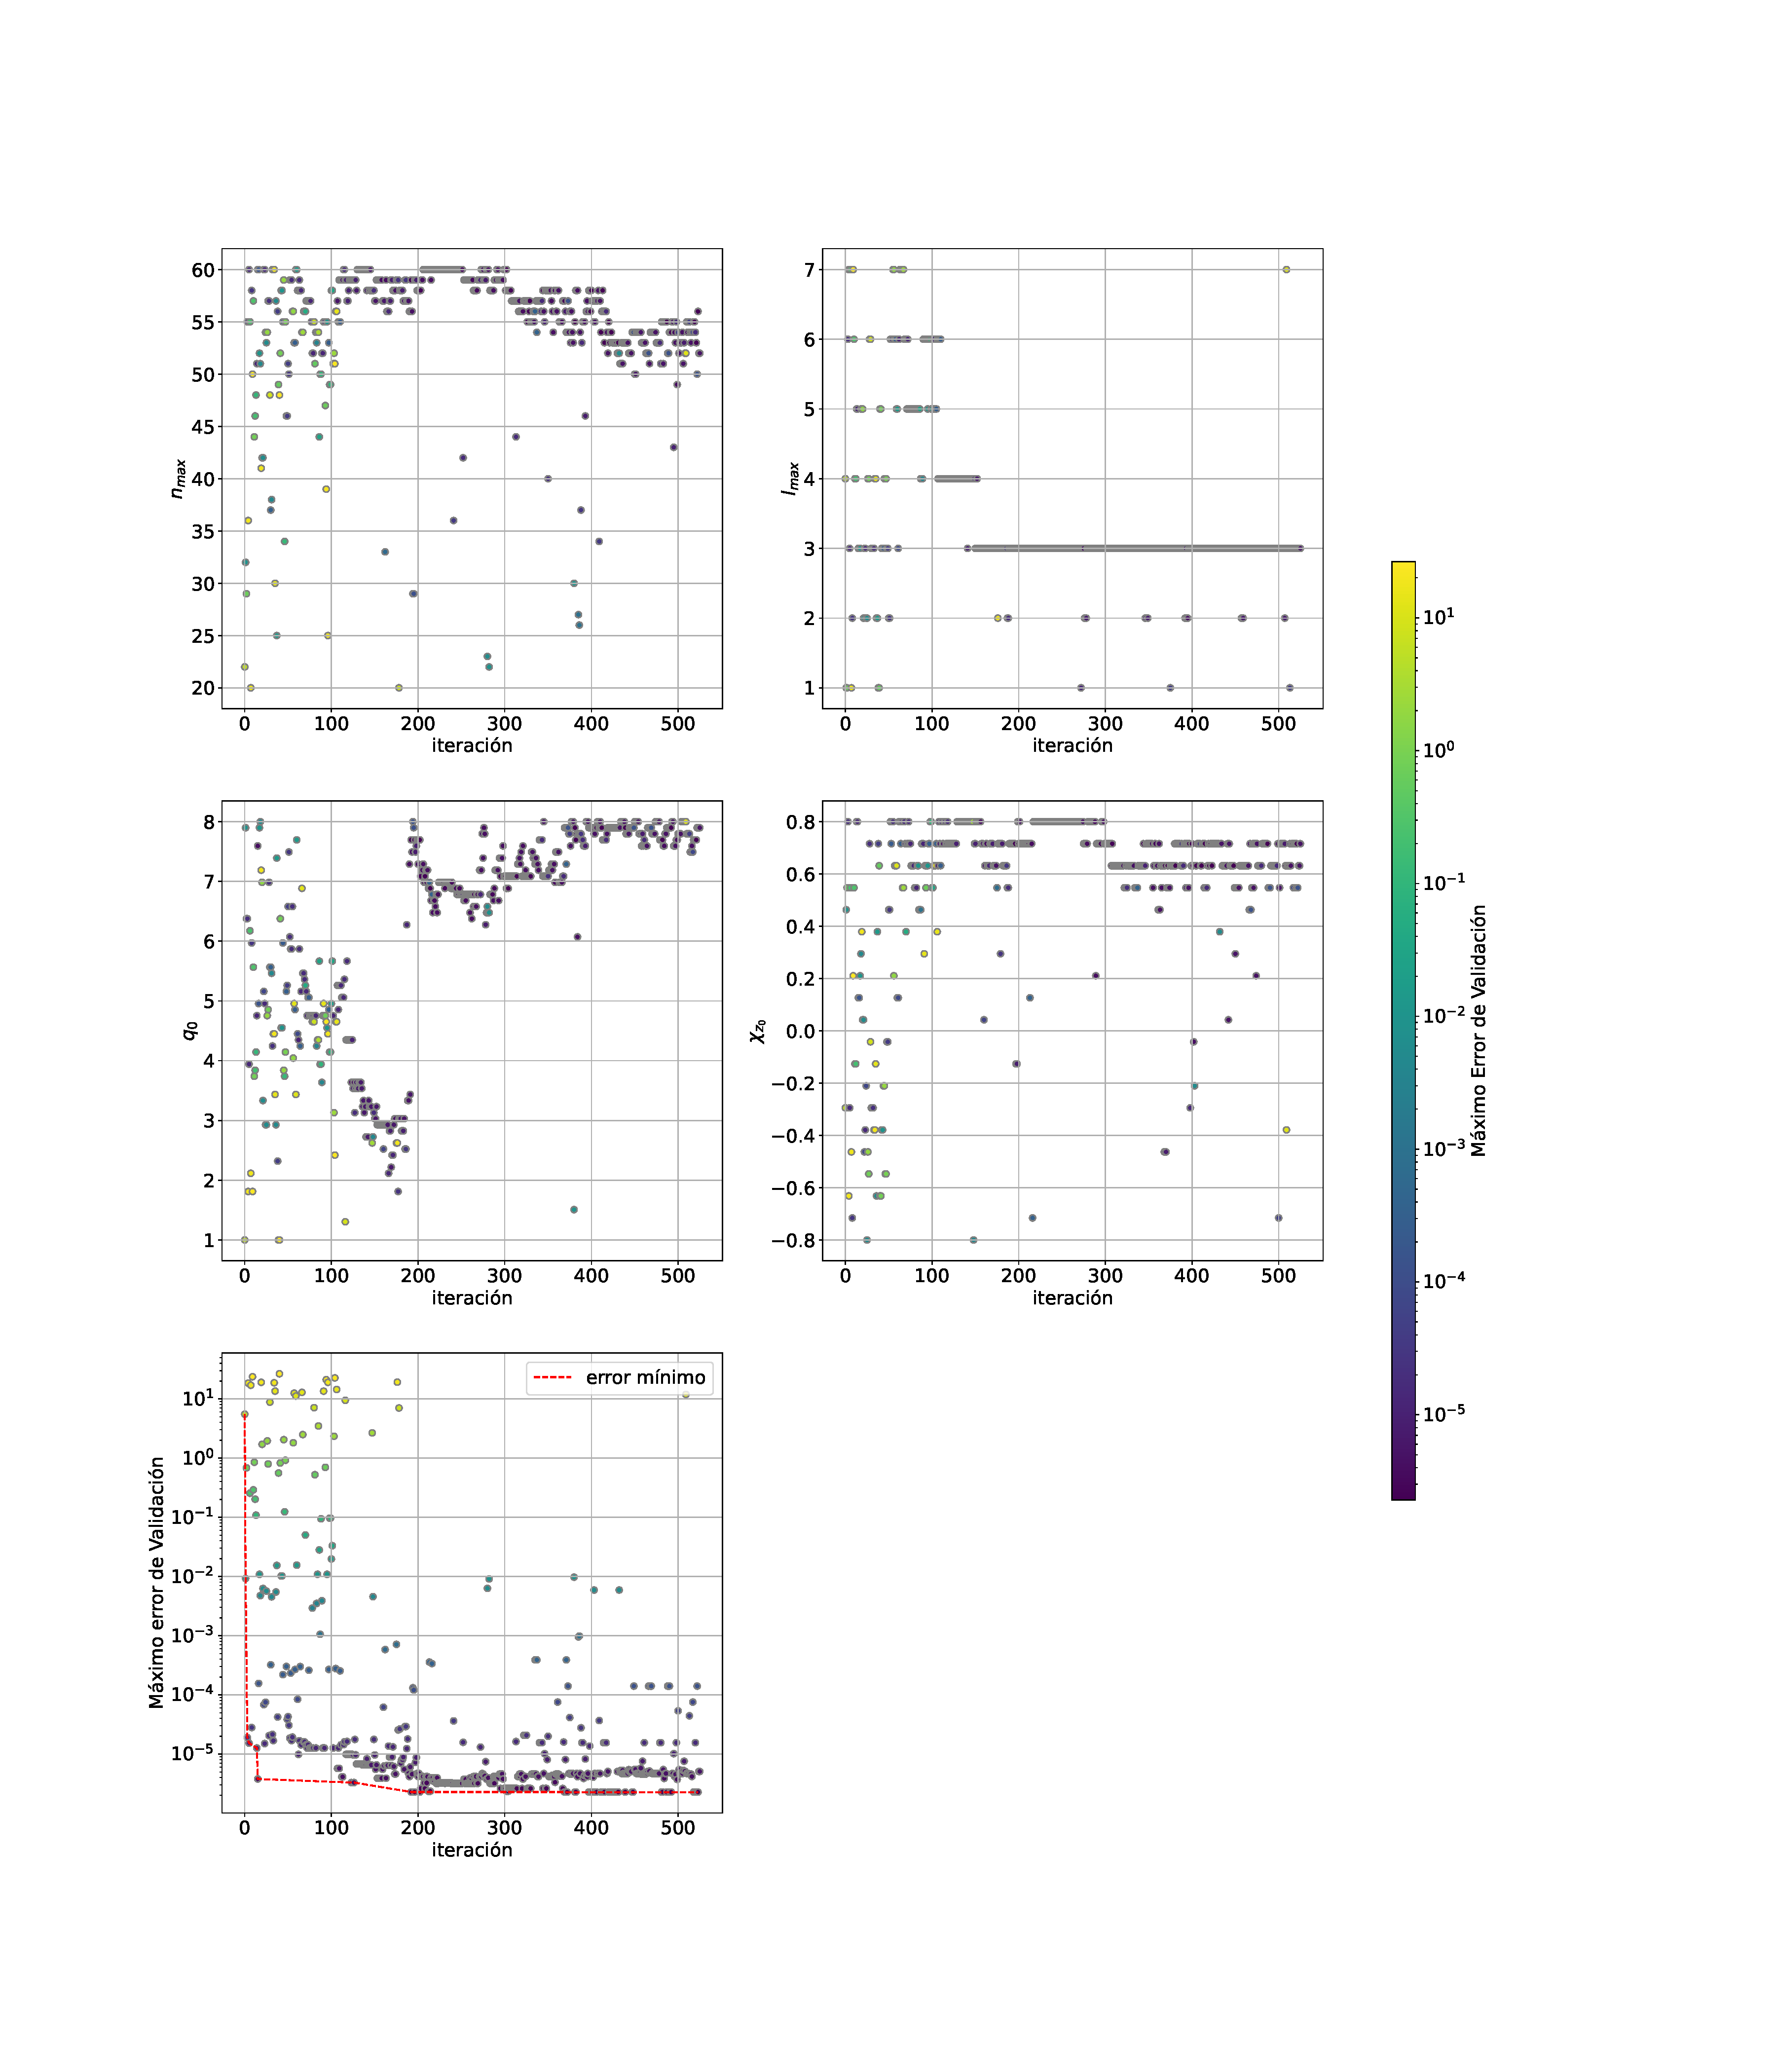
\includegraphics[width=1\columnwidth, trim={6cm, 5cm, 12cm, 5cm}]{Optuna_2D_noepsilon.pdf}
\caption{caption }
\label{fig:optuna_2d}
\end{figure}

\begin{figure}[p!]
\centering
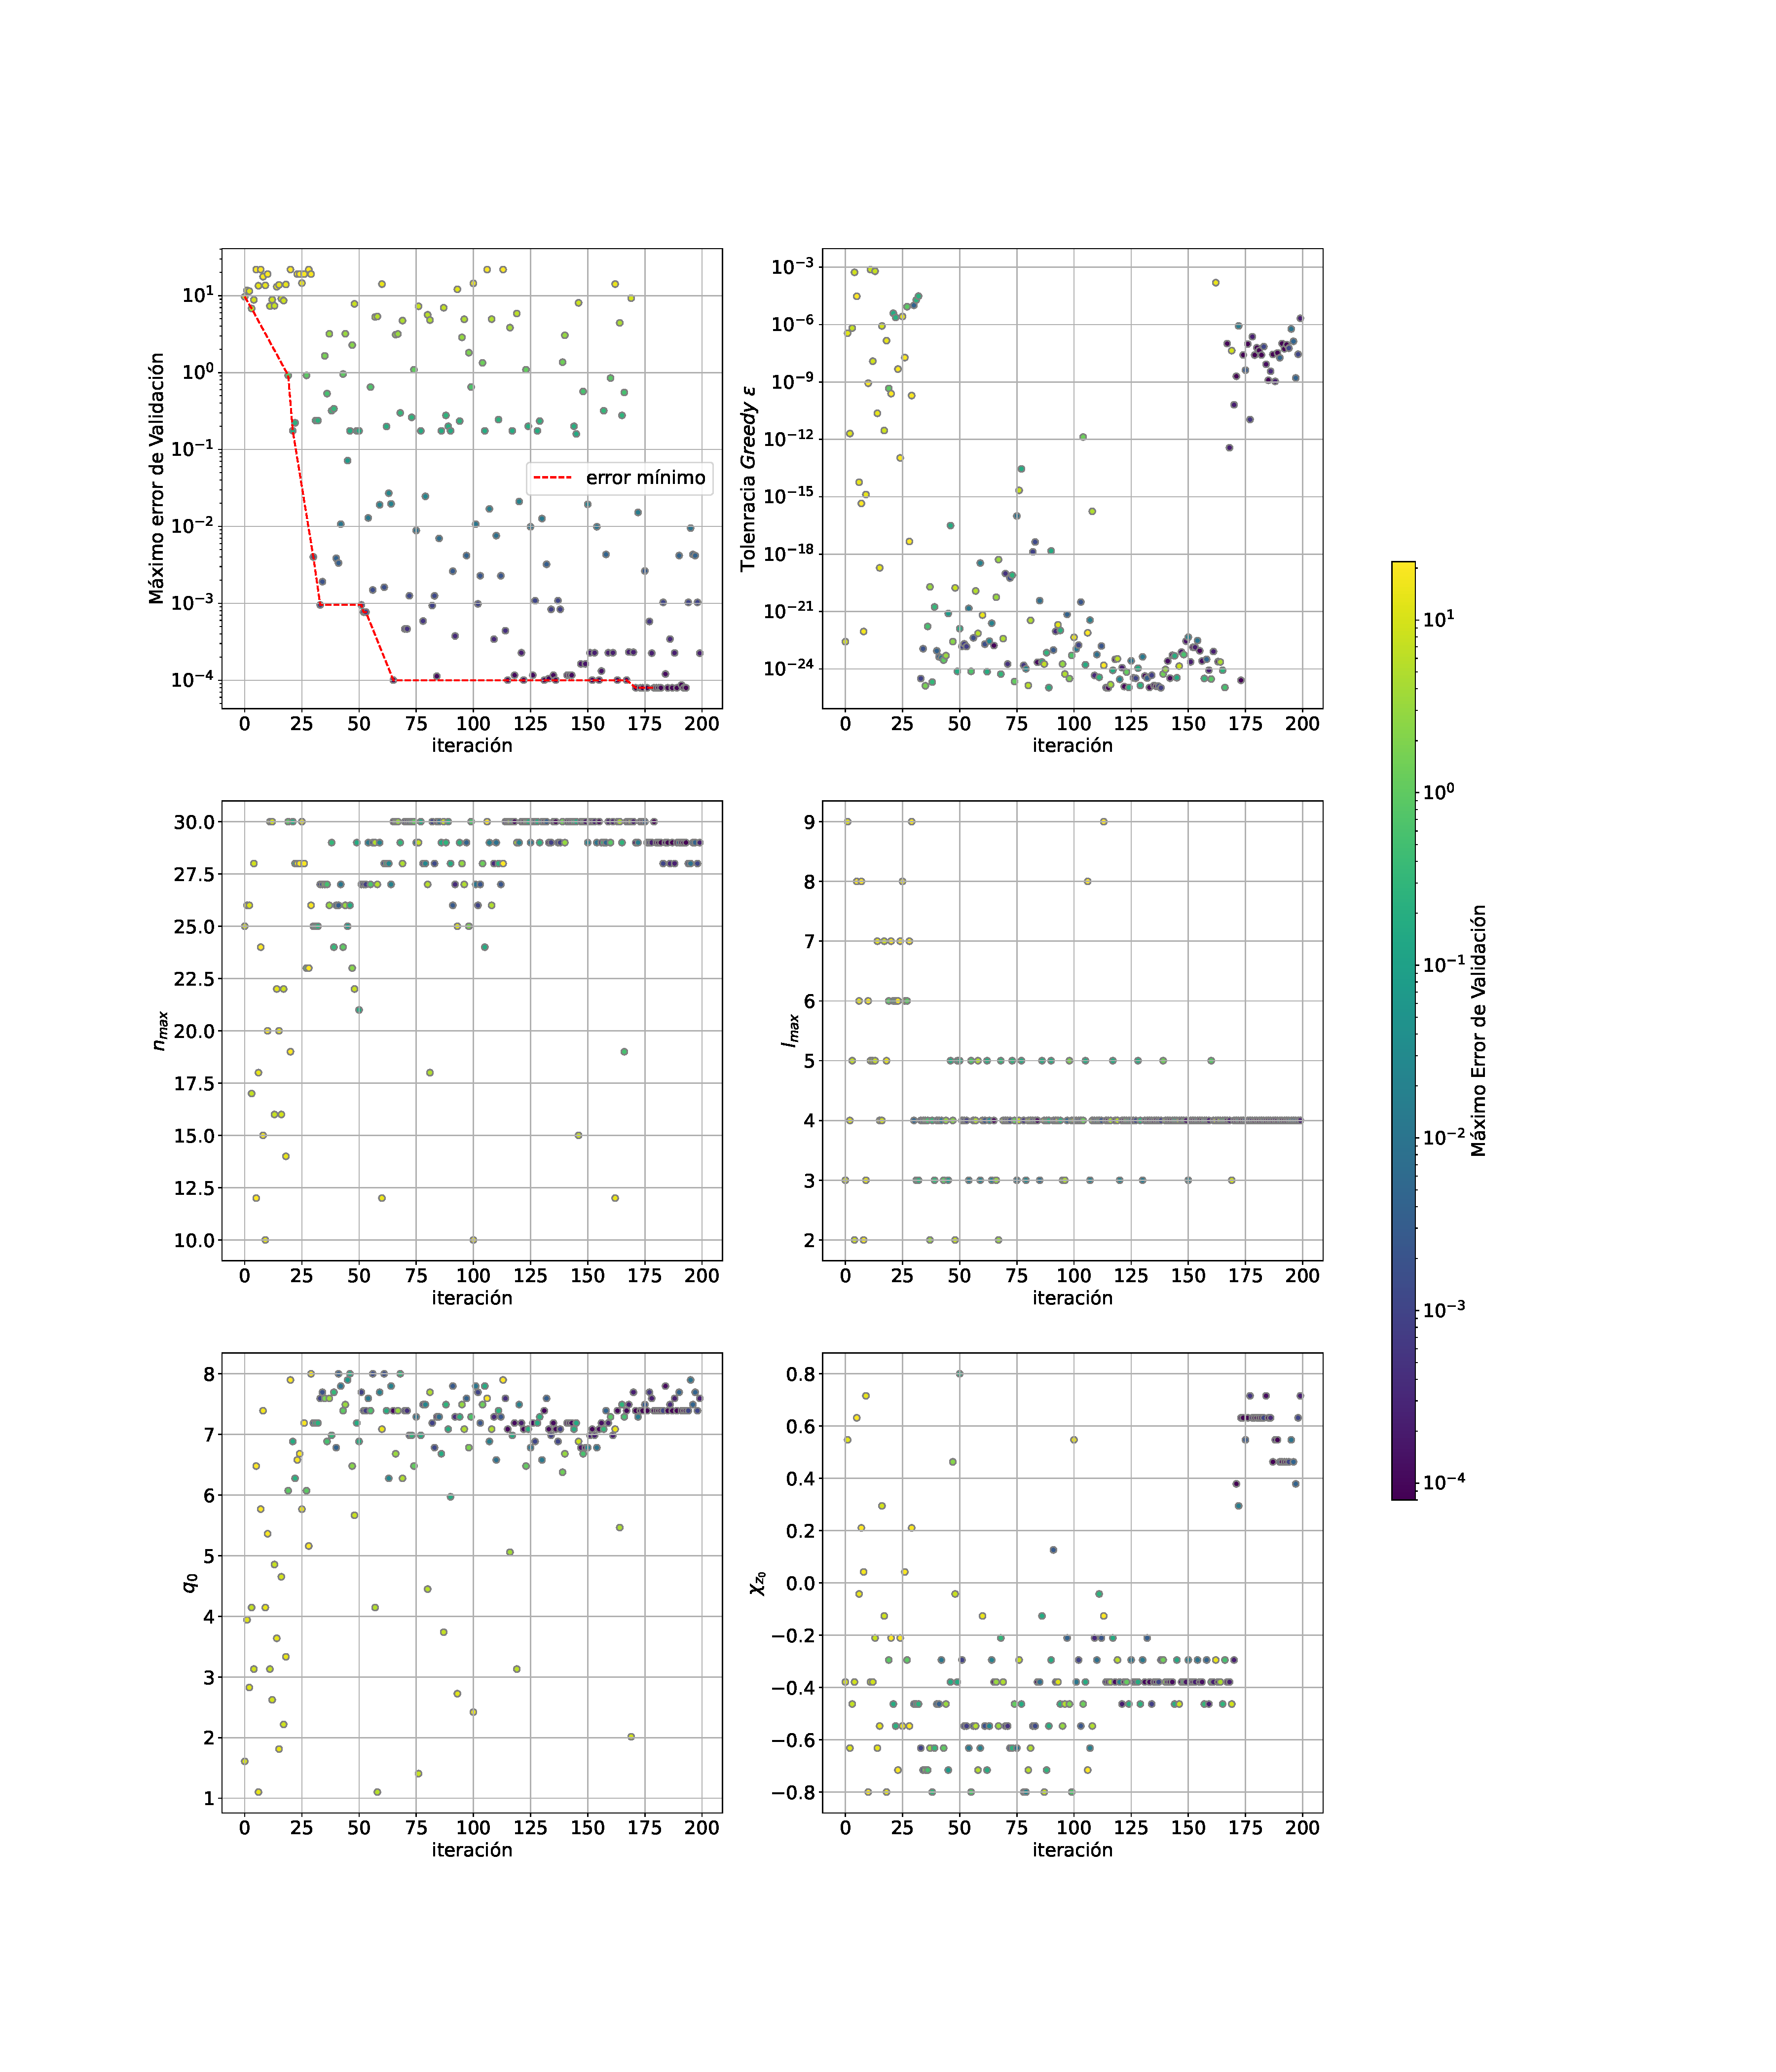
\includegraphics[width=1\columnwidth, trim={6cm, 5cm, 12cm, 5cm}]{Optuna_2D.pdf}
\caption{caption }
\label{fig:optuna_2d}
\end{figure}



\subsection{Importancia de los Hiperparámetros}

\appendix
%\include{apend1}

\begin{biblio}
\bibliography{mibib}
\end{biblio}


\begin{postliminary}

\begin{seccion}{Publicaciones asociadas}
  \begin{enumerate}
  \item Mi primer aviso en la revista \textbf{ABC}, 1996
  \item Mi segunda publicaci\'{o}n en la revista \textbf{ABC}, 1997
  \end{enumerate}
\end{seccion}

\begin{seccion}{Agradecimientos}
A todos los que se lo merecen, por merecerlo
\end{seccion}

\end{postliminary}

\end{document}

